\documentclass[a4paper,12pt]{report}
\usepackage{authblk}

% Codifica e lingua
\usepackage[utf8]{inputenc}
\usepackage[T1]{fontenc}
\usepackage[italian]{babel}

% Geometria pagina
\usepackage[margin=3cm]{geometry}

% Matematica
\usepackage{amsmath,amssymb,amsfonts}
\usepackage{amsthm}

% Tabelle ed array
\usepackage{array}
\usepackage{booktabs}     % Migliora le tabelle (riga orizz. professionali)

% Varie
\usepackage{stmaryrd}     % Simboli extra
\usepackage{fancyvrb}     % Verbatim avanzato
\usepackage{listings}     % Per listati di codice
\usepackage{xcolor}       % Colori
\usepackage{hyperref}     % Link ipertestuali nel PDF

% Grafica e disegni
\usepackage{graphicx}     % Inclusione immagini
\usepackage{tikz}         % Disegni con TikZ
\usetikzlibrary{arrows.meta,automata,positioning,shapes,%
                shapes.geometric,arrows} 
% NB: si possono aggiungere altre librerie in \usetikzlibrary come serve

% Stile pagina
\usepackage{fancyhdr}
\pagestyle{fancy}

% Esempio di definizione di uno stile personalizzato per i listati
\lstdefinestyle{arduinoStyle}{
  language=C++,                    % Riconosce la sintassi C++
  basicstyle=\ttfamily\small,      % Font 'typewriter' più piccolo
  frame=single,                    % Cornice intorno al codice
  backgroundcolor=\color{gray!10}, % Colore di sfondo (grigio chiaro)
  keywordstyle=\bfseries\color{blue},     % Parole chiave in blu e grassetto
  commentstyle=\itshape\color{teal},      % Commenti in corsivo color 'teal'
  stringstyle=\color{magenta},            % Stringhe in magenta
  showstringspaces=false,                 % Non mostra spazi nelle stringhe
  numbers=left,                           % Numeri di linea a sinistra
  numberstyle=\tiny\color{gray},         % Stile dei numeri di linea
  breaklines=true,                        % Va a capo automaticamente
  captionpos=b,                           % Didascalia in basso
}

\newcommand{\Xd}[1]{\mathrm{X_{#1}}}  % Esempio: \Xd{3} -> X_{3}
\newcommand{\Sd}[1]{\mathrm{S_{#1}}}  % Esempio: \Sd{7} -> S_{7}


% Header and footer
\lhead{Modulo 1 - Fondamenti di Informatica}
\rhead{Corso STEM}
\cfoot{\thepage}

% Title
\title{\textbf{Modulo 1: Introduzione al Calcolo Automatico e Fondamenti di Informatica}}
\author[1]{Francesco Sisini}
\author[2]{Lisa Galvani} % Considerato come collaboratore
\author[3]{Annalisa Pazzi} % Considerato come collaboratore

\affil[1]{Docente esperto di informatica e matematica applicate alle STEM}
\affil[2]{Tutor corsi STEM}
\affil[3]{Consulenza artistica e creativa}
\date{}

\begin{document}
\small
\maketitle
\chapter{Teoria degli automi}
\section*{Introduzione storica al concetto di calcolo automatico}

L'idea di calcolo automatico affonda le sue radici nel XVII secolo con il filosofo e matematico \textbf{Gottfried Wilhelm Leibniz}, che concepì la possibilità di una \textit{“macchina di ragionamento”} capace di eseguire calcoli logici e matematici in modo meccanico. Questi concetti furono formalizzati nel corso dei secoli successivi, culminando con l'introduzione del \textbf{calcolo simbolico} e degli \textbf{algoritmi} come strumenti fondamentali per automatizzare operazioni ripetitive.

Con l'avvento del XX secolo, \textbf{Alan Turing} diede un contributo decisivo, introducendo la \textbf{Macchina di Turing}, un modello astratto che rappresenta qualsiasi calcolo eseguibile tramite un algoritmo. Questo concetto segnò la nascita della \textit{teoria del calcolo} e gettò le basi per la creazione dei moderni computer.

Parallelamente, l'interesse per la formalizzazione dei linguaggi, attraverso la grammatica e la logica, portò allo sviluppo della \textbf{teoria dei linguaggi formali}. Autori come \textbf{Noam Chomsky} classificarono i linguaggi in gerarchie, legando il concetto di linguaggio a quello di automi.

Infine, grazie ai lavori pionieristici di \textbf{Claude Shannon}, nacque la \textbf{teoria dell'informazione}, che definì formalmente il concetto di \textit{informazione}, compressione dei dati e trasmissione efficiente dei messaggi, elementi alla base delle tecnologie digitali moderne.

Dalle intuizioni di Leibniz alle odierne applicazioni dell'informatica, il calcolo automatico, il linguaggio e la teoria dell'informazione hanno trasformato radicalmente la nostra capacità di risolvere problemi e comunicare, rappresentando il fondamento del mondo digitale contemporaneo.


\section*{Concetto di Automa e Classificazione secondo Chomsky}
\subsection*{Cos'\`e un Automa?}
Un \textbf{automa} \`e un modello matematico che rappresenta un sistema capace di eseguire calcoli o riconoscere linguaggi tramite una serie di stati e transizioni. Esso \`e un concetto fondamentale in informatica teorica e automazione.

Gli automi possono essere rappresentati attraverso:
\begin{itemize}
    \item Stati (finito o infinito).
    \item Simboli di ingresso (alfabeto).
    \item Transizioni tra stati.
\end{itemize}

Un automa riceve un input (sequenza di simboli) e si muove tra stati seguendo regole definite. Il comportamento \`e deterministico (determinato) o non deterministico (scelte multiple).

\subsection*{Classificazione degli Automi secondo Chomsky}
La classificazione di Chomsky distingue quattro tipi principali di automi, ciascuno capace di riconoscere linguaggi diversi:
\begin{enumerate}
    \item \textbf{Automi a Stati Finiti (Finite State Automata - FSA)}: Riconoscono linguaggi regolari. Non hanno memoria esterna e si limitano a muoversi tra stati finiti.
    \item \textbf{Automi a Pila (Pushdown Automata - PDA)}: Riconoscono linguaggi liberi dal contesto. Dispongono di una memoria a pila.
    \item \textbf{Macchine di Turing}: Riconoscono linguaggi ricorsivamente enumerabili. Dispongono di un nastro infinito che funge da memoria.
    \item \textbf{Automi Lineari Limitati (Linear Bounded Automata - LBA)}: Variante della Macchina di Turing con memoria limitata.
\end{enumerate}

\subsection*{Esempio: Automa a Stati Finiti}
Consideriamo un \textbf{Automa a Stati Finiti Deterministico (DFA)} che riconosce stringhe composte da simboli \{0, 1\} e che terminano con il simbolo "1".

\subsubsection*{Definizione Formale}
L'automa \`e definito dalla quintupola $(Q, \Sigma, \delta, q_0, F)$ dove:
\begin{itemize}
    \item $Q$: Insieme degli stati, $Q = \{q_0, q_1\}$.
    \item $\Sigma$: Alfabeto, $\Sigma = \{0, 1\}$.
    \item $\delta$: Funzione di transizione.
    \item $q_0$: Stato iniziale.
    \item $F$: Stato finale, $F = \{q_1\}$.
\end{itemize}

\subsubsection*{Tabella di Transizione}
\begin{center}
\begin{tabular}{|c|c|c|}
    \hline
    Stato & Input & Nuovo Stato \\
    \hline
    $q_0$ & 0 & $q_0$ \\
    $q_0$ & 1 & $q_1$ \\
    $q_1$ & 0 & $q_0$ \\
    $q_1$ & 1 & $q_1$ \\
    \hline
\end{tabular}
\end{center}

\subsubsection*{Schema Grafico dell'Automa}
\begin{center}
\begin{tikzpicture}[node distance=2cm, auto, every state/.style={draw, circle}]
    \node[state, initial] (q0) {$q_0$};
    \node[state, accepting, right of=q0] (q1) {$q_1$};

    \draw[->] (q0) edge[loop above] node{0} (q0);
    \draw[->] (q0) edge[bend left] node{1} (q1);
    \draw[->] (q1) edge[loop above] node{1} (q1);
    \draw[->] (q1) edge[bend left] node{0} (q0);
\end{tikzpicture}
\end{center}

\subsubsection*{Esempio di Esecuzione}
Se l'input \`e la stringa $1011$:
\begin{itemize}
    \item Stato iniziale: $q_0$.
    \item Legge $1$: passa a $q_1$.
    \item Legge $0$: torna a $q_0$.
    \item Legge $1$: va a $q_1$.
    \item Legge $1$: rimane a $q_1$.
    \item Stato finale: $q_1$ (accettazione).
\end{itemize}

La stringa viene accettata perch\'e termina in "1".


\section*{Lezione 1: Macchina di Turing e il Concetto di Calcolo Automatico}
\subsection*{Obiettivi}
\begin{itemize}
    \item Comprendere il concetto di algoritmo e computabilit\`a.
    \item Conoscere la figura di Alan Turing e il funzionamento della Macchina di Turing.
    \item Sviluppare algoritmi semplici manualmente.
\end{itemize}

\subsection*{La Macchina di Turing}
La Macchina di Turing \`e un modello astratto di calcolatore ideato da Alan Turing per rappresentare il processo di calcolo automatico. Consiste in:
\begin{itemize}
    \item Un nastro infinito diviso in celle, che rappresenta la memoria.
    \item Una testina di lettura/scrittura che si sposta sul nastro.
    \item Uno stato interno che indica il "programma" attualmente eseguito.
    \item Una tabella di transizione che definisce le azioni della macchina in base allo stato e al simbolo letto.
\end{itemize}

\subsection*{Esempio: Somma di Numeri Interi (0-10)}
Supponiamo di sommare due numeri interi compresi tra 0 e 10, rappresentati in formato unario:
\begin{itemize}
    \item 2 \`e rappresentato come $11$, 3 come $111$.
    \item La macchina sposta i simboli "1" del primo gruppo accanto al secondo gruppo.
\end{itemize}

\textbf{Tabella delle Transizioni per la Somma Aritmetica}
\begin{center}
\begin{tabular}{|c|c|c|c|c|}
    \hline
    Stato & Simbolo Letto & Scrivi & Movimento & Nuovo Stato \\
    \hline
    $q_0$ & 1 & \_ & Destra & $q_1$ \\
    $q_1$ & \_ & 1 & Destra & $q_1$ \\
    $q_1$ & 1 & 1 & Destra & $q_1$ \\
    $q_1$ & \_ & \_ & Sinistra & $q_2$ \\
    $q_2$ & 1 & 1 & Sinistra & $q_2$ \\
    $q_2$ & \_ & \_ & Stop & Halt \\
    \hline
\end{tabular}
\end{center}

\textbf{Risultato Finale:} Il nastro conterr\`a i due gruppi di "1" concatenati, rappresentando la somma unaria.

\subsection*{Schema della Macchina di Turing}
\begin{center}
\begin{tikzpicture}[node distance=1.5cm, auto]
    \node (nastro) [rectangle, draw, minimum height=1cm, minimum width=5cm] {Nastro Infinito (Memoria)};
    \node (testina) [circle, draw, below=of nastro, minimum size=1cm] {Testina};
    \node (stato) [rectangle, draw, below=of testina, minimum height=1cm, minimum width=3cm] {Stato Interno};
    \node (transizione) [rectangle, draw, below=of stato, minimum height=1cm, minimum width=4cm] {Tabella Transizioni};

    \draw [->] (nastro) -- (testina);
    \draw [->] (testina) -- (stato);
    \draw [->] (stato) -- (transizione);
\end{tikzpicture}
\end{center}

\newpage
\section*{Lezione 2: Architettura Base del Computer}
\subsection*{Obiettivi}
\begin{itemize}
    \item Comprendere la struttura interna di un computer.
    \item Conoscere i componenti principali: ALU, CPU, registri e memoria.
    \item Simulare il funzionamento della CPU con un esempio pratico.
\end{itemize}

\subsection*{Registri Principali}
I registri sono celle di memoria velocissime interne alla CPU. Ecco i registri principali:
\begin{itemize}
    \item \textbf{Registro Istruzione (IR)}: Contiene l'istruzione attualmente in esecuzione.
    \item \textbf{Program Counter (PC)}: Tiene traccia dell'indirizzo della prossima istruzione da eseguire.
    \item \textbf{Accumulator (ACC)}: Usato per operazioni aritmetiche e logiche.
    \item \textbf{Registro Dati (DR)}: Contiene i dati temporanei utilizzati durante l'elaborazione.
\end{itemize}

\subsection*{Schema dell'Architettura della CPU}
\begin{center}
\begin{tikzpicture}[node distance=1.5cm, auto]
    \node (input) [rectangle, draw, text centered, minimum height=1cm, minimum width=2cm] {Input};
    \node (memory) [rectangle, draw, right=of input, minimum height=1cm, minimum width=2cm] {Memoria Principale};
    \node (cpu) [rectangle, draw, below=of memory, minimum height=1cm, minimum width=2cm] {CPU};
    \node (alu) [rectangle, draw, below=of cpu, minimum height=1cm, minimum width=2cm] {ALU};
    \node (output) [rectangle, draw, right=of memory, minimum height=1cm, minimum width=2cm] {Output};

    \draw [->] (input) -- (memory);
    \draw [->] (memory) -- (cpu);
    \draw [->] (cpu) -- (alu);
    \draw [->] (alu) -- (cpu);
    \draw [->] (memory) -- (output);
\end{tikzpicture}
\end{center}
\newpage

\section*{Esempio: Automa a Stati Finiti per un Ascensore Semplice}
Un automa a stati finiti per un ascensore semplice si basa su un modello deterministico (DFA) che gestisce solo l'apertura e la chiusura delle porte e il movimento tra i piani. Non ha memoria dei piani visitati in precedenza.

\subsubsection*{Definizione Formale}
L'automa può essere definito dalla quintupola $(Q, \Sigma, \delta, q_0, F)$ dove:
\begin{itemize}
    \item $Q = \{\text{Idle}, \text{Moving}, \text{Open}\}$: Stati possibili.
    \item $\Sigma = \{\text{Up}, \text{Down}, \text{OpenDoor}, \text{CloseDoor}\}$: Input possibili.
    \item $\delta$: Funzione di transizione definita da una tabella (vedi sotto).
    \item $q_0 = \text{Idle}$: Stato iniziale.
    \item $F = \{\text{Idle}\}$: Stato finale (opzionale, quando l'ascensore è inattivo).
\end{itemize}

\subsubsection*{Tabella di Transizione}
\begin{center}
\begin{tabular}{|c|c|c|}
    \hline
    Stato Attuale & Input & Nuovo Stato \\
    \hline
    \text{Idle} & \text{Up} & \text{Moving} \\
    \text{Idle} & \text{Down} & \text{Moving} \\
    \text{Idle} & \text{OpenDoor} & \text{Open} \\
    \text{Moving} & \text{Stop} & \text{Idle} \\
    \text{Open} & \text{CloseDoor} & \text{Idle} \\
    \hline
\end{tabular}
\end{center}

\subsubsection*{Schema Grafico dell'Automa}
\begin{center}
\begin{tikzpicture}[node distance=4cm, auto, every state/.style={draw, circle}]
    \node[state, initial] (idle) {Idle};
    \node[state, right of=idle] (moving) {Moving};
    \node[state, below of=idle] (open) {Open};

    \draw[->] (idle) edge[below] node{OpenDoor} (open);
    \draw[->] (idle) edge[bend left] node{Up, Down} (moving);
    \draw[->] (moving) edge[bend left] node{Stop} (idle);
    \draw[->] (open) edge[bend above] node{CloseDoor} (idle);
\end{tikzpicture}
\end{center}

\newpage

\section*{Esempio: Automa a Pila per un Ascensore con Memoria del Piano}
Un automa a pila (PDA) consente di tenere traccia dei piani visitati utilizzando una pila per memorizzare le sequenze di piani. Questo modello è utile per ascensori che ricordano i piani richiesti e visitati in ordine.

\subsubsection*{Definizione Formale}
L'automa è definito da $(Q, \Sigma, \Gamma, \delta, q_0, Z_0, F)$ dove:
\begin{itemize}
    \item $Q = \{\text{Idle}, \text{Moving}, \text{Open}\}$: Stati possibili.
    \item $\Sigma = \{\text{Up}, \text{Down}, \text{OpenDoor}, \text{CloseDoor}, \text{Request(n)}\}$: Input possibili.
    \item $\Gamma = \{\text{1}, \text{2}, \text{3}, \dots, Z_0\}$: Alfabeto della pila (piani richiesti).
    \item $\delta$: Funzione di transizione (vedi sotto).
    \item $q_0 = \text{Idle}$: Stato iniziale.
    \item $Z_0$: Simbolo iniziale della pila.
    \item $F = \{\text{Idle}\}$: Stato finale (opzionale, quando l'ascensore è inattivo).
\end{itemize}

\subsubsection*{Funzione di Transizione}
Le transizioni aggiungono piani alla pila e li rimuovono quando vengono visitati.
\begin{align*}
\delta(q, \text{Request(n)}, Z) &= (q, \text{Push(n)}) \\
\delta(\text{Moving}, \text{Arrived(n)}, n) &= (\text{Open}, \text{Pop()})
\end{align*}

\subsubsection*{Tabella di Transizione}
\begin{center}
\begin{tabular}{|c|c|c|c|}
    \hline
    Stato Attuale & Input & Simbolo Pila & Nuovo Stato / Azione \\
    \hline
    \text{Idle} & \text{Request(n)} & $Z_0$ & \text{Idle, Push(n)} \\
    \text{Idle} & \text{Up, Down} & n & \text{Moving} \\
    \text{Moving} & \text{Arrived(n)} & n & \text{Open, Pop()} \\
    \text{Open} & \text{CloseDoor} & - & \text{Idle} \\
    \hline
\end{tabular}
\end{center}

\subsubsection*{Schema Grafico dell'Automa}
\begin{center}
\begin{tikzpicture}[node distance=2cm, auto, every state/.style={draw, circle}]
    \node[state, initial] (idle) {Idle};
    \node[state, right of=idle] (moving) {Moving};
    \node[state, below of=moving] (open) {Open};

    \draw[->] (idle) edge[loop above] node{Request(n), Push(n)} (idle);
    \draw[->] (idle) edge[bend left] node{Up, Down} (moving);
    \draw[->] (moving) edge[bend left] node{Arrived(n), Pop()} (open);
    \draw[->] (open) edge[bend left] node{CloseDoor} (idle);
\end{tikzpicture}
\end{center}

\section*{Spiegazione del Funzionamento dell'Automa a Pila}

L'automa a pila per l'ascensore con memoria del piano utilizza una struttura dati a pila per ricordare i piani richiesti. Ogni volta che un piano viene richiesto, il numero del piano viene aggiunto alla pila. Quando l'ascensore raggiunge un piano, il numero del piano viene rimosso dalla pila. Questo meccanismo consente all'ascensore di tenere traccia dell'ordine dei piani da visitare, in base alle richieste degli utenti.

\subsection*{Dettaglio del Funzionamento}
\begin{enumerate}
    \item \textbf{Richiesta di un Piano:} Quando un utente richiede di andare a un piano (\texttt{Request(n)}), l'automa passa allo stato \texttt{Idle}, mantenendo il piano richiesto nella pila tramite l'operazione di \textit{Push(n)}.
    \item \textbf{Movimento:} Una volta che l'ascensore inizia a muoversi verso un piano (\texttt{Up} o \texttt{Down}), l'automa entra nello stato \texttt{Moving}.
    \item \textbf{Arrivo al Piano:} Quando l'ascensore raggiunge un piano specifico (\texttt{Arrived(n)}), verifica che il piano corrisponda al valore in cima alla pila. Se corrisponde, il numero viene rimosso dalla pila tramite l'operazione \textit{Pop()}, e l'automa passa allo stato \texttt{Open}.
    \item \textbf{Apertura e Chiusura delle Porte:} Lo stato \texttt{Open} indica che le porte dell'ascensore sono aperte. Dopo che le porte vengono chiuse (\texttt{CloseDoor}), l'automa torna allo stato \texttt{Idle}.
    \item \textbf{Verifica della Pila:} L'automa controlla se la pila è vuota. Se lo è, l'ascensore rimane nello stato \texttt{Idle}. In caso contrario, prosegue verso il prossimo piano in cima alla pila.
\end{enumerate}

\subsection*{Esempio di Esecuzione}
Consideriamo un esempio pratico:
\begin{itemize}
    \item Un utente richiede i piani 3 e 5 in quest'ordine (\texttt{Request(3)} e \texttt{Request(5)}).
    \item La pila inizialmente contiene il simbolo iniziale $Z_0$. Dopo le richieste, la pila sarà: [$Z_0$, 5, 3].
    \item L'ascensore si muove (\texttt{Up}) e raggiunge il piano 3 (\texttt{Arrived(3)}). Il piano 3 viene rimosso dalla pila tramite \textit{Pop()}, lasciando la pila con [$Z_0$, 5].
    \item Dopo aver aperto e chiuso le porte, l'ascensore riparte verso il piano 5. Al suo arrivo (\texttt{Arrived(5)}), il piano 5 viene rimosso dalla pila, che ritorna allo stato iniziale [$Z_0$].
    \item L'automa ritorna allo stato \texttt{Idle}, pronto per nuove richieste.
\end{itemize}

\subsection*{Vantaggi del Modello a Pila}
Questo modello consente di gestire in modo efficiente richieste multiple, garantendo che l'ascensore visiti i piani in ordine di richiesta. Inoltre, utilizza la pila per ricordare i piani ancora da visitare, evitando comportamenti incoerenti o disordinati.

\section*{Approfondimenti sul Funzionamento dell'Automa a Pila}

\subsection*{Come l'Automa Riconosce di Essere Giunto a un Piano}
L'automa sa di essere giunto a un determinato piano grazie a un segnale esterno, come un sensore installato in ciascun piano dell'edificio. Quando l'ascensore si ferma in corrispondenza del piano, il sensore invia un segnale all'automa, indicando il numero del piano. Questo segnale viene interpretato come l'input \texttt{Arrived(n)}.

Ad esempio:
\begin{itemize}
    \item Se l'ascensore si ferma al 3° piano, il sensore invia l'input \texttt{Arrived(3)}.
    \item L'automa confronta questo input con il simbolo in cima alla pila. Se il simbolo in cima è "3", l'automa conferma di essere giunto al piano richiesto e procede a rimuovere "3" dalla pila tramite l'operazione di \textit{Pop()}.
\end{itemize}

Questo meccanismo garantisce che l'automa non rimuova piani dalla pila in modo casuale, ma solo quando corrispondono al piano effettivamente raggiunto.

\subsection*{Esempio: Raggiungere un Piano Diverso dall'Ordine di Richiesta}
Consideriamo un esempio in cui l'ascensore riceve due richieste: prima per il 5° piano (\texttt{Request(5)}) e poi per il 3° piano (\texttt{Request(3)}). La pila viene gestita in ordine LIFO (Last In, First Out), quindi la richiesta per il piano 3 viene posizionata sopra quella per il piano 5.

\subsubsection*{Passaggi Eseguiti dall'Automa}
\begin{enumerate}
    \item \textbf{Stato Iniziale:} La pila contiene [$Z_0$, 5, 3]. L'automa si trova nello stato \texttt{Idle}.
    \item \textbf{Movimento verso il 3° piano:}
        \begin{itemize}
            \item L'ascensore inizia a muoversi (\texttt{Up}) verso il piano più vicino.
            \item Quando arriva al 3° piano, il sensore invia l'input \texttt{Arrived(3)}.
            \item L'automa verifica che il simbolo in cima alla pila sia "3". Poiché c'è corrispondenza, rimuove "3" dalla pila (\textit{Pop()}), lasciando la pila con [$Z_0$, 5].
        \end{itemize}
    \item \textbf{Apertura e Chiusura delle Porte al 3° piano:}
        \begin{itemize}
            \item L'automa passa allo stato \texttt{Open}, indicando che le porte sono aperte.
            \item Dopo che le porte si richiudono (\texttt{CloseDoor}), l'automa ritorna allo stato \texttt{Idle}.
        \end{itemize}
    \item \textbf{Movimento verso il 5° piano:}
        \begin{itemize}
            \item L'ascensore riparte verso il 5° piano.
            \item Quando arriva al 5° piano, il sensore invia l'input \texttt{Arrived(5)}.
            \item L'automa verifica che il simbolo in cima alla pila sia "5". Poiché c'è corrispondenza, rimuove "5" dalla pila (\textit{Pop()}), lasciando la pila con [$Z_0$].
        \end{itemize}
    \item \textbf{Apertura e Chiusura delle Porte al 5° piano:}
        \begin{itemize}
            \item L'automa passa allo stato \texttt{Open}, indicando che le porte sono aperte.
            \item Dopo che le porte si richiudono (\texttt{CloseDoor}), l'automa ritorna allo stato \texttt{Idle}.
        \end{itemize}
\end{enumerate}

\subsubsection*{Osservazioni Importanti}
\begin{itemize}
    \item L'automa non si preoccupa di eseguire le richieste in ordine di inserimento nella pila. Segue invece l'ordine LIFO, servendo prima il piano più vicino (in cima alla pila).
    \item Questo comportamento potrebbe essere subottimale in alcuni contesti reali, ma riflette accuratamente il modello di funzionamento di una pila (Last In, First Out).
\end{itemize}

\subsection*{Vantaggi e Limitazioni del Modello}
\begin{itemize}
    \item \textbf{Vantaggi:} La pila semplifica la gestione delle richieste e permette un controllo chiaro e deterministico dei piani visitati.
    \item \textbf{Limitazioni:} L'ordine LIFO potrebbe non essere ottimale in contesti con molte richieste, poiché i piani richiesti per primi potrebbero essere serviti per ultimi.
\end{itemize}

\chapter{Un Gioco Collaborativo con Arduino}
\label{cap:gioco}

\section{Introduzione}
Lo scopo di questo capitolo è presentare un semplice gioco basato su \textbf{automazione a stati finiti}, realizzato con \textbf{Arduino} e due pulsanti. Il gioco nasce come esempio di \textbf{gioco cooperativo} nell'ambito della \textbf{teoria dei giochi} di John von Neumann.

Il sistema prevede quattro stati principali, associati a quattro LED di colori diversi (Rosso \texttt{R}, Verde \texttt{G}, Blu \texttt{B}, Bianco \texttt{W}). A ogni pressione di un pulsante, il sistema cambia stato secondo una tabella di transizione concordata. L’obiettivo globale è produrre la sequenza 
\[
\text{W} \;\to\; \text{G} \;\to\; \text{R} \;\to\; \text{G} \;\to\; \text{R} \;\to\; \text{G} \;\to\; \text{B} \;\to\; \text{W},
\]
sequenza che, come vedremo, non può essere realizzata da un singolo giocatore, ma richiede la collaborazione di entrambi.

\section{Inquadramento nella teoria dei giochi}
La \emph{teoria dei giochi} di von Neumann analizza le decisioni strategiche di agenti (giocatori) che operano in un sistema di regole ben definito. Nei \emph{giochi competitivi}, ogni giocatore massimizza il proprio payoff individuale. Tuttavia, esistono anche \emph{giochi cooperativi} o collaborativi, dove due (o più) giocatori devono \emph{cooperare} per raggiungere un obiettivo comune.

Nel nostro caso:
\begin{itemize}
    \item I giocatori sono due \emph{persone} (due pulsanti).
    \item Non hanno interessi in conflitto: \textbf{entrambi} vogliono ottenere la sequenza desiderata.
    \item Di conseguenza, non siamo in presenza di una competizione a somma zero, bensì di un gioco \emph{collaborativo}.
\end{itemize}
Poiché la sequenza da produrre include alternanze di mosse (pressioni) da parte del ``giocatore 1'' e del ``giocatore 2'', un solo giocatore non può completare l’intero percorso. Serve necessariamente l’azione dell’altro.

\section{Modello come automa a stati finiti}
Formalmente, possiamo descrivere il sistema come un \textbf{automa a stati finiti}:
\begin{itemize}
    \item \(\Sigma = \{\, P_1, P_2\}\) è l'insieme degli \emph{ingressi} (pulsante 1 e pulsante 2).
    \item \(Q = \{\texttt{R}, \texttt{G}, \texttt{B}, \texttt{W}\}\) è l'insieme degli \emph{stati} (Rosso, Verde, Blu, Bianco).
    \item \(\delta\colon Q\times \Sigma \to Q\) è la funzione di transizione. Ad esempio:
      \[
        \delta(\texttt{R}, P_1) = \texttt{G}, \quad
        \delta(\texttt{R}, P_2) = \texttt{B},\quad \dots
      \]
      secondo la tabella di gioco concordata.
    \item \(q_0 = \texttt{R}\) è lo \emph{stato iniziale}.
\end{itemize}
Premendo i pulsanti (ingressi), i giocatori causano transizioni nello spazio degli stati. L’obiettivo di squadra è passare per una certa sequenza di stati (corrispondente ai colori dei LED) che \emph{non} è realizzabile da un singolo giocatore.

\section{Realizzazione con Arduino}
\subsection{Descrizione hardware}
La realizzazione hardware prevede:
\begin{itemize}
  \item Una scheda Arduino (ad es. Arduino UNO).
  \item Due pulsanti di input (\texttt{BUTTON1} e \texttt{BUTTON2}), ciascuno con una resistenza di \emph{pull-down} da 10 k\(\Omega\).
  \item Quattro LED (\texttt{RED\_LED}, \texttt{GREEN\_LED}, \texttt{BLUE\_LED}, \texttt{WHITE\_LED}) per indicare lo stato corrente.
\end{itemize}
Il pulsante 1 è collegato al pin digitale \texttt{2}, il pulsante 2 al pin \texttt{3}. I LED sono collegati a \texttt{9}, \texttt{10}, \texttt{11}, \texttt{12} rispettivamente (o a discrezione del progettista).

\subsection{Schema dei collegamenti}
In modo semplificato:
\begin{itemize}
  \item \(\texttt{BUTTON1}\): un capo a +5V, l’altro al pin \texttt{2}, e in parallelo una resistenza da 10 k\(\Omega\) tra il pin \texttt{2} e GND.
  \item \(\texttt{BUTTON2}\): un capo a +5V, l’altro al pin \texttt{3}, e in parallelo una resistenza da 10 k\(\Omega\) tra il pin \texttt{3} e GND.
  \item \(\texttt{RED\_LED}\): pin \texttt{9} \(\rightarrow\) Resistenza (220 \(\Omega\)) \(\rightarrow\) Anodo LED, catodo a GND.
  \item \(\texttt{GREEN\_LED}\), \(\texttt{BLUE\_LED}\), \(\texttt{WHITE\_LED}\) similmente, sui pin \texttt{10}, \texttt{11}, \texttt{12}.
\end{itemize}

\subsection{Codice di esempio}
Il seguente listato \ref{lst:gioco} implementa la logica di cambiamento di stato in base al pulsante premuto. Ogni volta che il giocatore 1 (pulsante su pin 2) preme, passiamo a un ``prossimo'' colore; se invece preme il giocatore 2 (pulsante su pin 3), la transizione segue la colonna dedicata a player 2. 

\begin{lstlisting}[style=arduinoStyle, caption={Codice Arduino}, label={lst:arduino}]
/****************************************************
 * Gioco collaborativo con 4 LED e 2 pulsanti
 * Basato su transizioni di stato distinte per P1 e P2
 ****************************************************/
// Pin LED
const int RED_LED = 9;
const int GREEN_LED = 10;
const int BLUE_LED = 11;
const int WHITE_LED = 12;

// Pin pulsanti (pull-down esterna)
const int BUTTON1 = 2;
const int BUTTON2 = 3;

// Stato iniziale
char currentState = 'R';  // Rosso

void setup() {
  Serial.begin(9600);
  pinMode(RED_LED,   OUTPUT);
  pinMode(GREEN_LED, OUTPUT);
  pinMode(BLUE_LED,  OUTPUT);
  pinMode(WHITE_LED, OUTPUT);

  pinMode(BUTTON1, INPUT);
  pinMode(BUTTON2, INPUT);

  // Spegne tutti i LED
  digitalWrite(RED_LED,   LOW);
  digitalWrite(GREEN_LED, LOW);
  digitalWrite(BLUE_LED,  LOW);
  digitalWrite(WHITE_LED, LOW);

  // Accende il LED iniziale
  updateLED(currentState);
  Serial.println("Gioco avviato. Stato iniziale: R (Rosso).");
}

void loop() {
  // Lettura dei pulsanti
  int stateButton1 = digitalRead(BUTTON1);
  int stateButton2 = digitalRead(BUTTON2);

  // Se pulsante 1 premuto
  if (stateButton1 == HIGH) {
    nextState(1);
    delay(200); // per evitare ripetizioni veloci
  }

  // Se pulsante 2 premuto
  if (stateButton2 == HIGH) {
    nextState(2);
    delay(200);
  }
}

// nextState: cambia stato a seconda del giocatore
void nextState(int player) {
  Serial.print("Stato attuale: ");
  Serial.print(currentState);
  Serial.print(" | Giocatore: ");
  Serial.println(player);

  if (currentState == 'R') {
    currentState = (player == 1) ? 'G' : 'B';
  }
  else if (currentState == 'G') {
    currentState = (player == 1) ? 'B' : 'R';
  }
  else if (currentState == 'B') {
    currentState = 'W'; // per entrambi i giocatori
  }
  else if (currentState == 'W') {
    currentState = (player == 1) ? 'R' : 'G';
  }

  Serial.print("Nuovo stato: ");
  Serial.println(currentState);

  updateLED(currentState);
}

// updateLED: spegne tutti e accende solo quello del colore corrente
void updateLED(char state) {
  digitalWrite(RED_LED,   LOW);
  digitalWrite(GREEN_LED, LOW);
  digitalWrite(BLUE_LED,  LOW);
  digitalWrite(WHITE_LED, LOW);

  switch(state) {
    case 'R': digitalWrite(RED_LED,   HIGH); break;
    case 'G': digitalWrite(GREEN_LED, HIGH); break;
    case 'B': digitalWrite(BLUE_LED,  HIGH); break;
    case 'W': digitalWrite(WHITE_LED, HIGH); break;
  }
}
\end{lstlisting}

\section{Proposta di ingegnerizzazione}
Come esercitazione di laboratorio, si può proporre agli studenti di:
\begin{enumerate}
  \item \textbf{Progettare il circuito stampato (PCB)}: partendo dallo schema elettrico (Arduino, due pulsanti, quattro LED), realizzare uno \emph{shield} o un PCB dedicato.  
  \item \textbf{Integrare un display o indicatori aggiuntivi}: mostrare la sequenza già realizzata e quella ancora necessaria per il completamento del gioco.  
  \item \textbf{Introdurre una temporizzazione o penalità}: ad esempio, se un giocatore preme troppo presto o troppo tardi, inserire meccanismi di \emph{timeout} e notifiche sonore.  
  \item \textbf{Analisi matematica di cooperazione}: quantificare il numero di \emph{mosse} necessarie per completare la sequenza e dimostrare che un giocatore da solo non può arrivare alla soluzione finale.
\end{enumerate}

\section{Conclusioni}
Abbiamo descritto un semplice \emph{automa a stati finiti} con \emph{quattro stati} (R, G, B, W) e \emph{due ingressi} (i pulsanti) che, premuti con opportune transizioni, possono realizzare una sequenza obiettivo che \textbf{richiede} la cooperazione di entrambi i giocatori. La natura \emph{collaborativa} del gioco lo inserisce pienamente fra i giochi cooperativi della teoria di von Neumann, evidenziando come in alcune situazioni i giocatori non siano \emph{concorrenti}, bensì \emph{alleati} verso un unico scopo.

Questo semplice prototipo può essere esteso e migliorato, offrendo numerose occasioni di riflessione e \emph{apprendimento pratico} sull’elettronica di base, sulla programmazione embedded e sulle implicazioni teoriche di cooperazione tra agenti.


% ------------------------------------------------------------------------------
% Definizioni di comodo per i simboli di pila, SENZA \texttt e SENZA underscore "nudo"
% ------------------------------------------------------------------------------
% In math mode, \Xd{3} produce "X_{3}" in un font tipografico matematico (roman).
% Se vuoi un altro font (sans-serif), puoi fare \mathsf al posto di \mathrm.

\chapter{Aritmetica e Logica Binaria}

\vspace{1em}
\noindent
\textbf{Indice dei Contenuti}  
1. Rappresentazione binaria \dotfill \pageref{sec:binaria} \\
2. Operazioni logiche (true e false) \dotfill \pageref{sec:logiche} \\
3. Aritmetica binaria (somma, sottrazione, moltiplicazione, divisione) \dotfill \pageref{sec:arit_bin} \\
4. Rappresentazione algebrica della logica (Algebra di Boole) \dotfill \pageref{sec:algebra_boole} \\
5. Aritmetica binaria con porte logiche \dotfill \pageref{sec:porte_logiche} \\
6. Aritmetica binaria implementata come un automa a pila (semplice) \dotfill \pageref{sec:automa_bin} \\
7. Aritmetica decimale implementata con un automa a pila (solo decenni) \dotfill \pageref{sec:automa_dec} \\

\newpage

\section{Rappresentazione binaria}\label{sec:binaria}
La \textbf{rappresentazione binaria} di un numero intero non negativo \(n\) è data da una sequenza di bit \((b_k b_{k-1} \dots b_1 b_0)\) tale che:
\[
n = \sum_{i=0}^k b_i \, 2^i,
\quad \text{dove ciascun } b_i \in \{0,1\}.
\]
Esempi:
\[
\begin{aligned}
13_{10} &= 1101_2,\\
5_{10}  &= 101_2,\\
0_{10}  &= 0_2,\\
1_{10}  &= 1_2.
\end{aligned}
\]

\subsection*{Tabella di alcuni numeri in binario/decimale}
\begin{center}
\renewcommand{\arraystretch}{1.2}
\begin{tabular}{c|c||c|c}
\toprule
\textbf{Decimale} & \textbf{Binario} & \textbf{Decimale} & \textbf{Binario}\\
\midrule
0 & 0 & 8  & 1000 \\
1 & 1 & 9  & 1001 \\
2 & 10 & 10 & 1010 \\
3 & 11 & 11 & 1011 \\
4 & 100 & 12 & 1100 \\
5 & 101 & 13 & 1101 \\
6 & 110 & 14 & 1110 \\
7 & 111 & 15 & 1111 \\
\bottomrule
\end{tabular}
\end{center}
Questa tabella estende i primi 16 numeri, evidenziando come ogni valore decimale corrisponda a univoca sequenza di bit.

\begin{figure}[H]
    \centering
    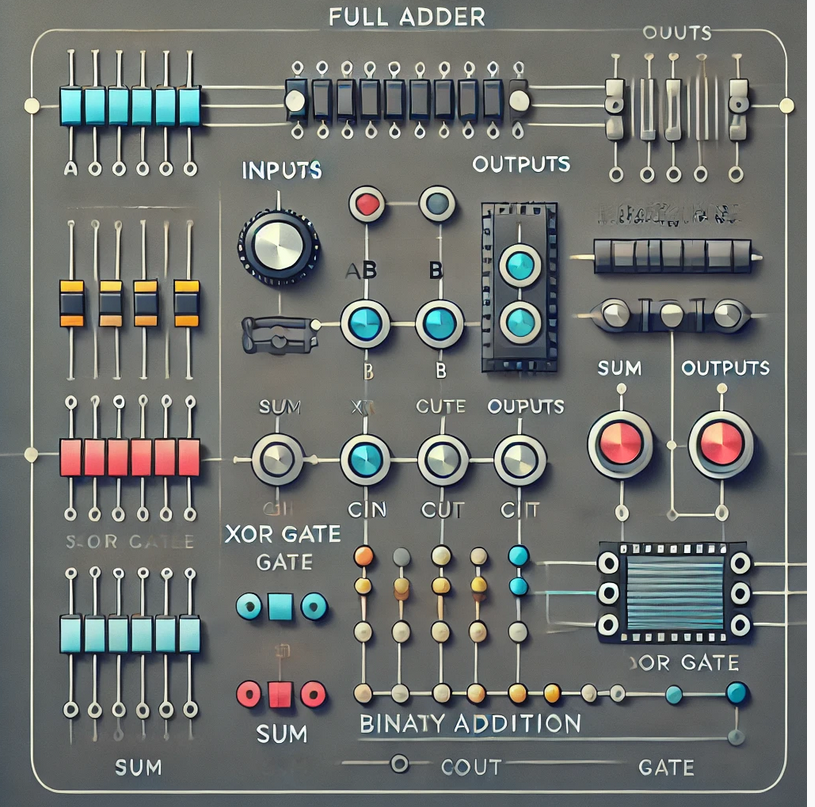
\includegraphics[width=0.8\textwidth]{fulladder.png}
    \caption{Diagramma del full adder binario: illustra in modo fantasioso le componenti principali, incluse le porte logiche XOR, AND e OR, con ingressi e uscite etichettate.}
    \label{fig:full_adder}
\end{figure}

\subsection*{Esercizi di Conversione}
\begin{enumerate}
    \item Converti i seguenti numeri decimali in binario: \(18, 20, 31, 32, 40, 50, 64, 100\).
    \item Converti da binario a decimale i seguenti numeri: \(10101_2, 100000_2, 111111_2, 1100100_2\).
    \item Spiega (in almeno 5-6 righe) come eseguire manualmente la conversione da decimale a binario, usando il metodo delle divisioni successive per 2.
\end{enumerate}

\newpage
\section{Operazioni logiche (true e false)}\label{sec:logiche}
La \textbf{logica booleana} ammette due valori: \(\text{TRUE}\) (vero) e \(\text{FALSE}\) (falso). Le \emph{operazioni fondamentali} sono:
\[
\land \ (\text{AND}),\quad
\lor \ (\text{OR}),\quad
\lnot \ (\text{NOT}).
\]
Le relative tabelle di verità sono:

\begin{center}
\renewcommand{\arraystretch}{1.2}
\begin{tabular}{c|c|c}
\multicolumn{3}{c}{\textbf{AND} (\(\land\))}\\
\hline
\(A\) & \(B\) & \(A \land B\) \\
\hline
F & F & F \\
F & T & F \\
T & F & F \\
T & T & T \\
\end{tabular}
\quad
\begin{tabular}{c|c|c}
\multicolumn{3}{c}{\textbf{OR} (\(\lor\))}\\
\hline
\(A\) & \(B\) & \(A \lor B\) \\
\hline
F & F & F \\
F & T & T \\
T & F & T \\
T & T & T \\
\end{tabular}
\quad
\begin{tabular}{c|c}
\multicolumn{2}{c}{\textbf{NOT} (\(\lnot\))}\\
\hline
\(A\) & \(\lnot A\) \\
\hline
F & T \\
T & F \\
\end{tabular}
\end{center}

\subsection*{Osservazioni}
\begin{itemize}
    \item L’operazione \(\land\) è “vera” solo se \emph{entrambe} le variabili d’ingresso sono vere.
    \item \(\lor\) è vera se almeno un operando è vero.
    \item \(\lnot\) inverte (NOT) il valore logico.
\end{itemize}

\subsection*{Esercizi di Logica}
\begin{enumerate}
    \item Verifica \((A \lor B) \land (A \lor \lnot B)\) per tutti i possibili valori di \(A,B\).
    \item Dimostra che \(\lnot(\lnot A) = A\) con la tabella di verità.
    \item Spiega che differenza c’è tra “AND esclusivo” (\(\oplus\)) e “AND” (\(\land\)).
\end{enumerate}

\newpage
\section{Aritmetica binaria: somma, sottrazione, moltiplicazione, divisione}\label{sec:arit_bin}
La \textbf{base 2} (\(\{0,1\}\)) richiede di gestire i riporti (o prestiti) in base 2.

\subsection{Somma binaria}
\[
0 + 0 = 0,\quad
0 + 1 = 1,\quad
1 + 0 = 1,\quad
1 + 1 = 0 \ \ (\text{con riporto }=1).
\]
Esempio: \((1001)_2 + (0110)_2 = (1111)_2\).

\subsection{Tabella di somma binaria (2 bit + carry)}
\[
\begin{array}{c|c|c||c|c}
x & y & c_{in} & s & c_{out} \\
\hline
0 & 0 & 0 & 0 & 0 \\
0 & 0 & 1 & 1 & 0 \\
0 & 1 & 0 & 1 & 0 \\
0 & 1 & 1 & 0 & 1 \\
1 & 0 & 0 & 1 & 0 \\
1 & 0 & 1 & 0 & 1 \\
1 & 1 & 0 & 0 & 1 \\
1 & 1 & 1 & 1 & 1 \\
\end{array}
\]
Questa tabella mostra tutte le combinazioni di due bit \(x,y\) e un carry in ingresso \(c_{in}\), e restituisce un bit di somma \(s\) e un carry in uscita \(c_{out}\).

\subsection{Sottrazione binaria}
Analogamente, se facciamo \((x - y)\), dobbiamo gestire il \emph{borrow} (prestito). Esempio: \((1000)_2 - (1)_2 = (0111)_2\).

\subsection{Moltiplicazione e divisione binaria}
Come in base 10, ma tutti i calcoli parziali usano bit.  
\[
(101)_2 \times (11)_2 = (1111)_2, \quad
(1100)_2 \div (10)_2 = (110)_2, \dots
\]

\subsection*{Esercizi Aritmetici}
\begin{enumerate}
    \item Somma in binario: \((1011)_2 + (0101)_2\), \((1111)_2 + (0001)_2\).
    \item Sottrai: \((10000)_2 - (0111)_2\).
    \item Moltiplica: \((101)_2 \times (101)_2\).  
    \item Dividi: \((1110)_2 \div (10)_2\).  
    \item Riporta in decimale i risultati e controlla la correttezza.
\end{enumerate}


\section{Rappresentazione algebrica della logica (Algebra di Boole)}\label{sec:algebra_boole}
L’\textbf{Algebra di Boole} utilizza i valori \(\{0,1\}\) con le operazioni \(\land\) (AND), \(\lor\) (OR), \(\lnot\) (NOT).  
Le \emph{leggi di De Morgan} affermano:
\[
\lnot(A \land B) = (\lnot A)\lor(\lnot B), \quad
\lnot(A \lor B) = (\lnot A)\land(\lnot B).
\]
Altre leggi fondamentali:
\[
A \land 1 = A,\quad
A \land 0 = 0,\quad
A \lor 1 = 1,\quad
A \lor 0 = A,\quad
(A \land B)\land C = A\land(B\land C), \ \dots
\]

\subsection*{Tabella di Verità per De Morgan}
\begin{center}
\renewcommand{\arraystretch}{1.2}
\begin{tabular}{ccc|c|c}
\toprule
$A$ & $B$ & $\lnot (A \land B)$ & $\lnot A \lor \lnot B$ & \text{Coincidenti?}\\
\midrule
0 & 0 & 1 & 1 & Sì\\
0 & 1 & 1 & 1 & Sì\\
1 & 0 & 1 & 1 & Sì\\
1 & 1 & 0 & 0 & Sì\\
\bottomrule
\end{tabular}
\end{center}
Si vede che \(\lnot(A \land B)\) e \((\lnot A)\lor(\lnot B)\) danno gli stessi risultati.

\subsection*{Esercizi di Algebra Booleana}
\begin{enumerate}
    \item Semplifica \(A \land (A \lor B)\) usando le leggi di assorbimento.  
    \item Riscrivi \(\lnot(A \lor (B \land C))\) usando De Morgan.
    \item Dimostra che \((A \land B) \land C = A \land (B \land C)\) (associatività).
\end{enumerate}


\section{Aritmetica binaria con porte logiche}\label{sec:porte_logiche}
Le operazioni binarie si implementano con \textbf{porte logiche}. Esempio: un \emph{full adder} somma due bit \(x,y\) più un carry in ingresso \(c_{in}\), restituendo la somma \(s\) e il carry in uscita \(c_{out}\).

\begin{center}
\begin{tabular}{c|c|c|c|c}
\toprule
$x$ & $y$ & $c_{in}$ & $s$ (somma) & $c_{out}$ (riporto)\\
\midrule
0 & 0 & 0 & 0 & 0 \\
0 & 0 & 1 & 1 & 0 \\
0 & 1 & 0 & 1 & 0 \\
0 & 1 & 1 & 0 & 1 \\
1 & 0 & 0 & 1 & 0 \\
1 & 0 & 1 & 0 & 1 \\
1 & 1 & 0 & 0 & 1 \\
1 & 1 & 1 & 1 & 1 \\
\bottomrule
\end{tabular}
\end{center}
Con \emph{porte XOR, AND, OR} si realizza questo comportamento:
\[
\begin{cases}
s = (x \oplus y) \oplus c_{in},\\
c_{out} = (x \land y) \lor \bigl( (x \oplus y)\land c_{in}\bigr).
\end{cases}
\]

\subsection*{Esempio di somma di 4 bit}
Usando 4 full adders in cascata (uno per ciascuna posizione), si ottiene la somma di due numeri binari di 4 bit. Il carry in uscita di un full adder diventa il carry in ingresso di quello sulla cifra più significativa successiva.

\subsection*{Esercizi sulle porte logiche}
\begin{enumerate}
    \item Disegna la porta \(\text{XOR}\) (o \text{EX-OR}) e spiega la differenza tra \(\text{XOR}\) e \(\text{OR}\).
    \item Calcola manualmente \((1011)_2 + (0101)_2\) usando la logica dei carry in ingresso e in uscita.
    \item Progetta un \emph{half adder} (somma di 2 bit senza carry in ingresso) e scrivi la relativa tabella di verità.
\end{enumerate}


\section{Aritmetica binaria implementata come un automa a pila (semplice)}\label{sec:automa_bin}
Mostriamo come un \emph{automa a pila} (PDA) riconosca correttamente \(\,x + y = z\) in base 2, assumendo che le cifre siano lette “\emph{rovesciate}” (cifra meno significativa per prima).

\subsection*{Fasi principali}
\begin{enumerate}
    \item \textbf{Caricamento \(x\)}: leggiamo i bit di \(x\) e li empiliamo come simboli (ad es.\ \(\mathrm{X\_0}\) o \(\mathrm{X\_1}\)).
    \item \textbf{Lettura \(y\)} e calcolo parziale: ogni volta che leggiamo un bit di \(y\), pop di un bit di \(x\) e somma binaria + carry. In cima alla pila spingiamo la cifra di somma (\(\mathrm{S\_0}\) o \(\mathrm{S\_1}\)), mentre il carry (0 o 1) viene memorizzato nello \emph{stato} dell’automa.
    \item \textbf{Verifica di \(z\)}: confrontiamo i bit di \(z\) letti con la somma parziale presente in cima alla pila.
    \item Accettiamo se, alla fine, la pila è vuota e il carry=0.
\end{enumerate}

\subsection*{Esempio: Somma \(101 + 11 = 1000\)}
In “forma rovesciata” diventa \(101 + 11 = 0001\) (da destra a sinistra!). L’automa:
\begin{itemize}
    \item Carica \(101\) in pila (\(\mathrm{X\_1}, \mathrm{X\_0}, \mathrm{X\_1}\)).
    \item Legge \(11\), bit a bit, somma e produce la “somma parziale” in pila.
    \item Verifica che \(0001\) corrisponda al risultato.  
\end{itemize}
In decimale, \(5 + 3 = 8\).

\subsection*{Esercizi}
\begin{enumerate}
    \item Scrivi la forma rovesciata di \(100 + 11 = 111\) e verifica i passaggi.
    \item Descrivi almeno due stati diversi dell’automa: uno per la lettura di \(x\), uno per la lettura di \(y\).  
    \item Spiega perché un automa a stati finiti \emph{senza pila} non è sufficiente a riconoscere correttamente tutte le somme binarie.
\end{enumerate}


\section{Aritmetica decimale implementata con un automa a pila (solo decenni)}\label{sec:automa_dec}
Analogamente, \textbf{in base 10} (decimale) possiamo costruire un automa a pila che riconosca espressioni come \(x + y = z\). Naturalmente, la gestione del \emph{carry} va da \(0\) a \(1\) (per due cifre 0--9 la somma può arrivare a 18), ma il principio è lo stesso.

\subsection*{Schema}
\begin{enumerate}
    \item Caricamento di \(x\) (cifre 0--9) in pila come \(\mathrm{X\_digit}\).
    \item Lettura di \(y\) e somma delle cifre: pop di \(\mathrm{X\_digit}\) e, con lo stato che memorizza carry 0 o 1, calcoliamo la cifra di somma (\(\mathrm{S\_digit}\)) e lo spingiamo in pila.
    \item Infine, verifichiamo \(z\) confrontando le cifre (lette in forma rovesciata) con quelle in cima alla pila.
    \item Accettiamo se la pila torna vuota e il carry finale è 0.
\end{enumerate}

\subsection*{Esempio}
\[
12 + 5 = 17 \quad\Rightarrow\quad \text{rovesciato: }21 + 5 = 71.
\]
In cifre rovesciate:
\begin{itemize}
    \item Carichiamo \(2\) e \(1\) in pila (come \(\mathrm{X\_2}\) e \(\mathrm{X\_1}\)).
    \item Leggiamo “\(5\)” per \(y\) e sommiamo \(\mathrm{X\_2}\) (in cima) con 5 più carry=0, ecc.
    \item Verifichiamo \(7\) e \(1\) nel risultato.
\end{itemize}

\subsection*{Esercizi}
\begin{enumerate}
    \item Rovescia \(123 + 45 = 168\) e spiega come funziona il carry (0 o 1).
    \item Disegna una piccola porzione di tabella di transizione, per lo stato “lettura di \(y\), carry=1” e cima della pila = \(\mathrm{X\_7}\).  
    \item Argomenta (in 5 righe) se servono stati diversi per carry=0 e carry=1.
\end{enumerate}

\section*{Conclusioni Generali}
Abbiamo visto:
\begin{itemize}
    \item La \textbf{rappresentazione binaria} e come essa sia la base dell’informatica.
    \item Le \textbf{operazioni logiche} \(\land, \lor, \lnot\) e l’algebra di Boole, fondamentali per l’elettronica digitale.
    \item L’\textbf{aritmetica binaria} (con esempi di somma, sottrazione, moltiplicazione e divisione).
    \item L’uso delle \textbf{porte logiche} per realizzare fisicamente tali operazioni (full adder, half adder, etc.).
    \item Come un \textbf{automa a pila} possa riconoscere “\(\,x+y=z\)” sia in base 2 sia in base 10, \emph{rovesciando} le cifre e memorizzandone alcune in pila.
\end{itemize}

\bigskip
\noindent
\textbf{Ulteriori spunti:}
\begin{itemize}
    \item Estendere il concetto all’algebra booleana di più variabili (circuiti con più ingressi).
    \item Analizzare la costruzione di una \emph{piccola CPU} con sommatore binario a 8 bit.
    \item Verificare se per la \emph{moltiplicazione in base 10} si può costruire un automa a pila simile (spoiler: si può, ma è più complesso).
\end{itemize}


%######################################


\chapter{Algoritmo di Somma e Architettura a Stati Finiti}

\section{Introduzione}
In questo capitolo descriveremo in dettaglio l'algoritmo di somma mostrato nel diagramma di flusso e nell'architettura schematica, soffermandoci su un esempio in \textbf{binario}. L'obiettivo è comprendere come i registri (quali \texttt{RC}, \texttt{ACC}, \texttt{AR}, \texttt{RI}, ecc.) interagiscano con l'Unità Aritmetico-Logica (ALU) e con la memoria dati per svolgere l'operazione di addizione di due operandi, bit per bit, gestendo correttamente il riporto (\texttt{carry}).

\begin{figure}[ht]
    \centering
    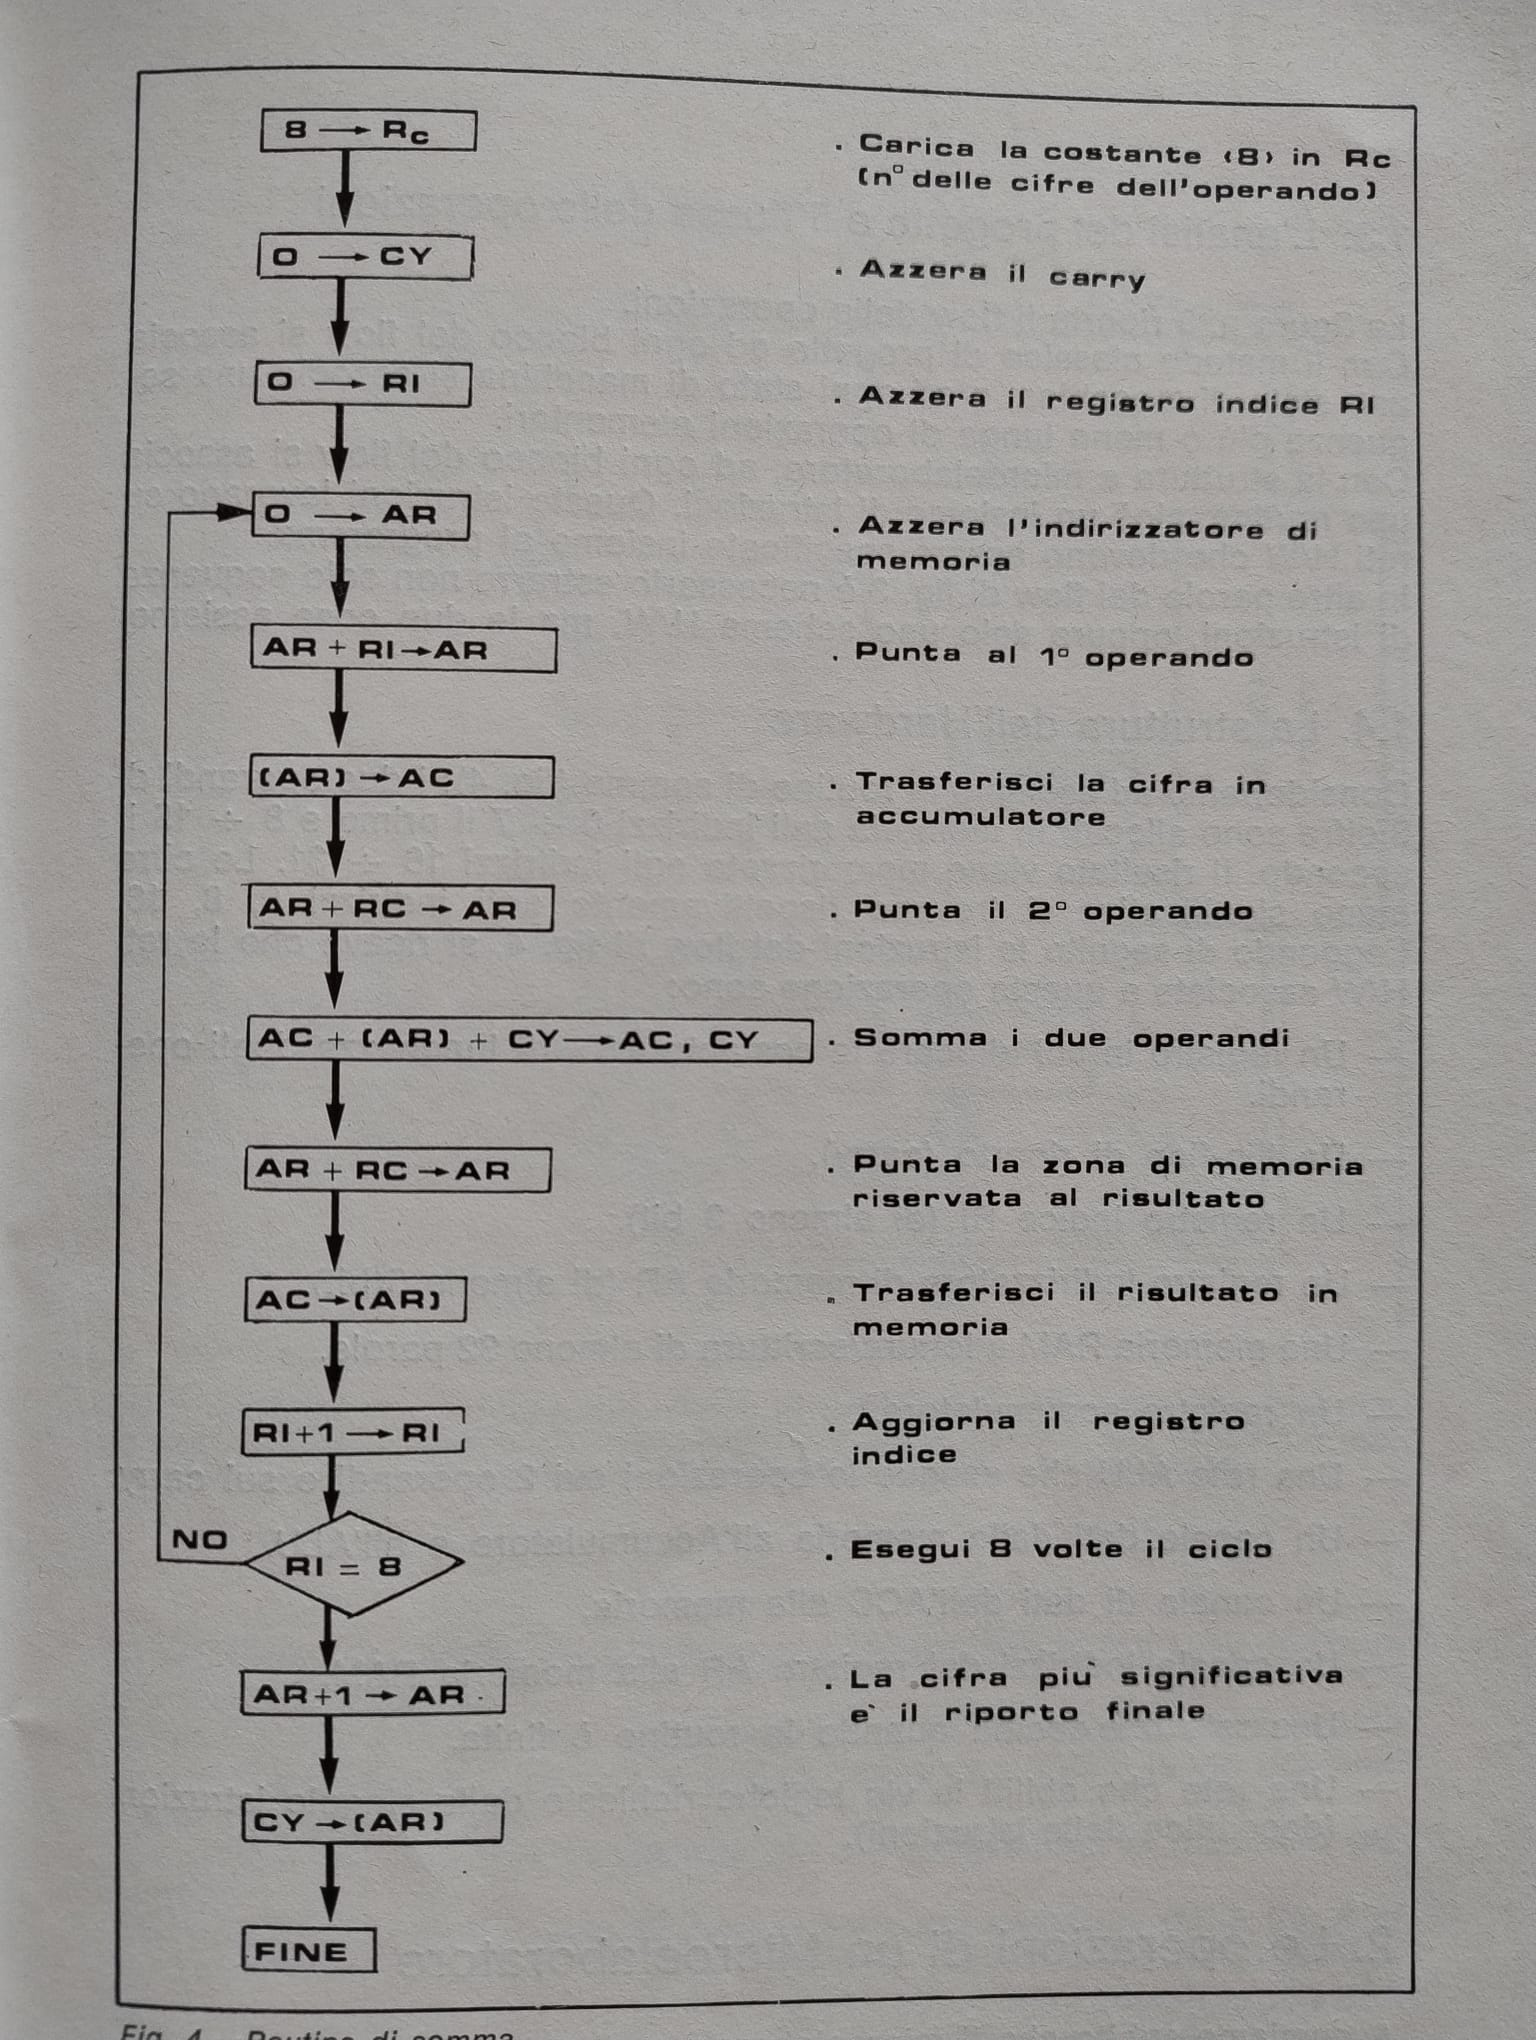
\includegraphics[width=0.6\textwidth]{algoritmo.jpeg}
    \caption{Diagramma di flusso dell'algoritmo di somma.}
    \label{fig:algoritmo}
\end{figure}

\begin{figure}[ht]
    \centering
    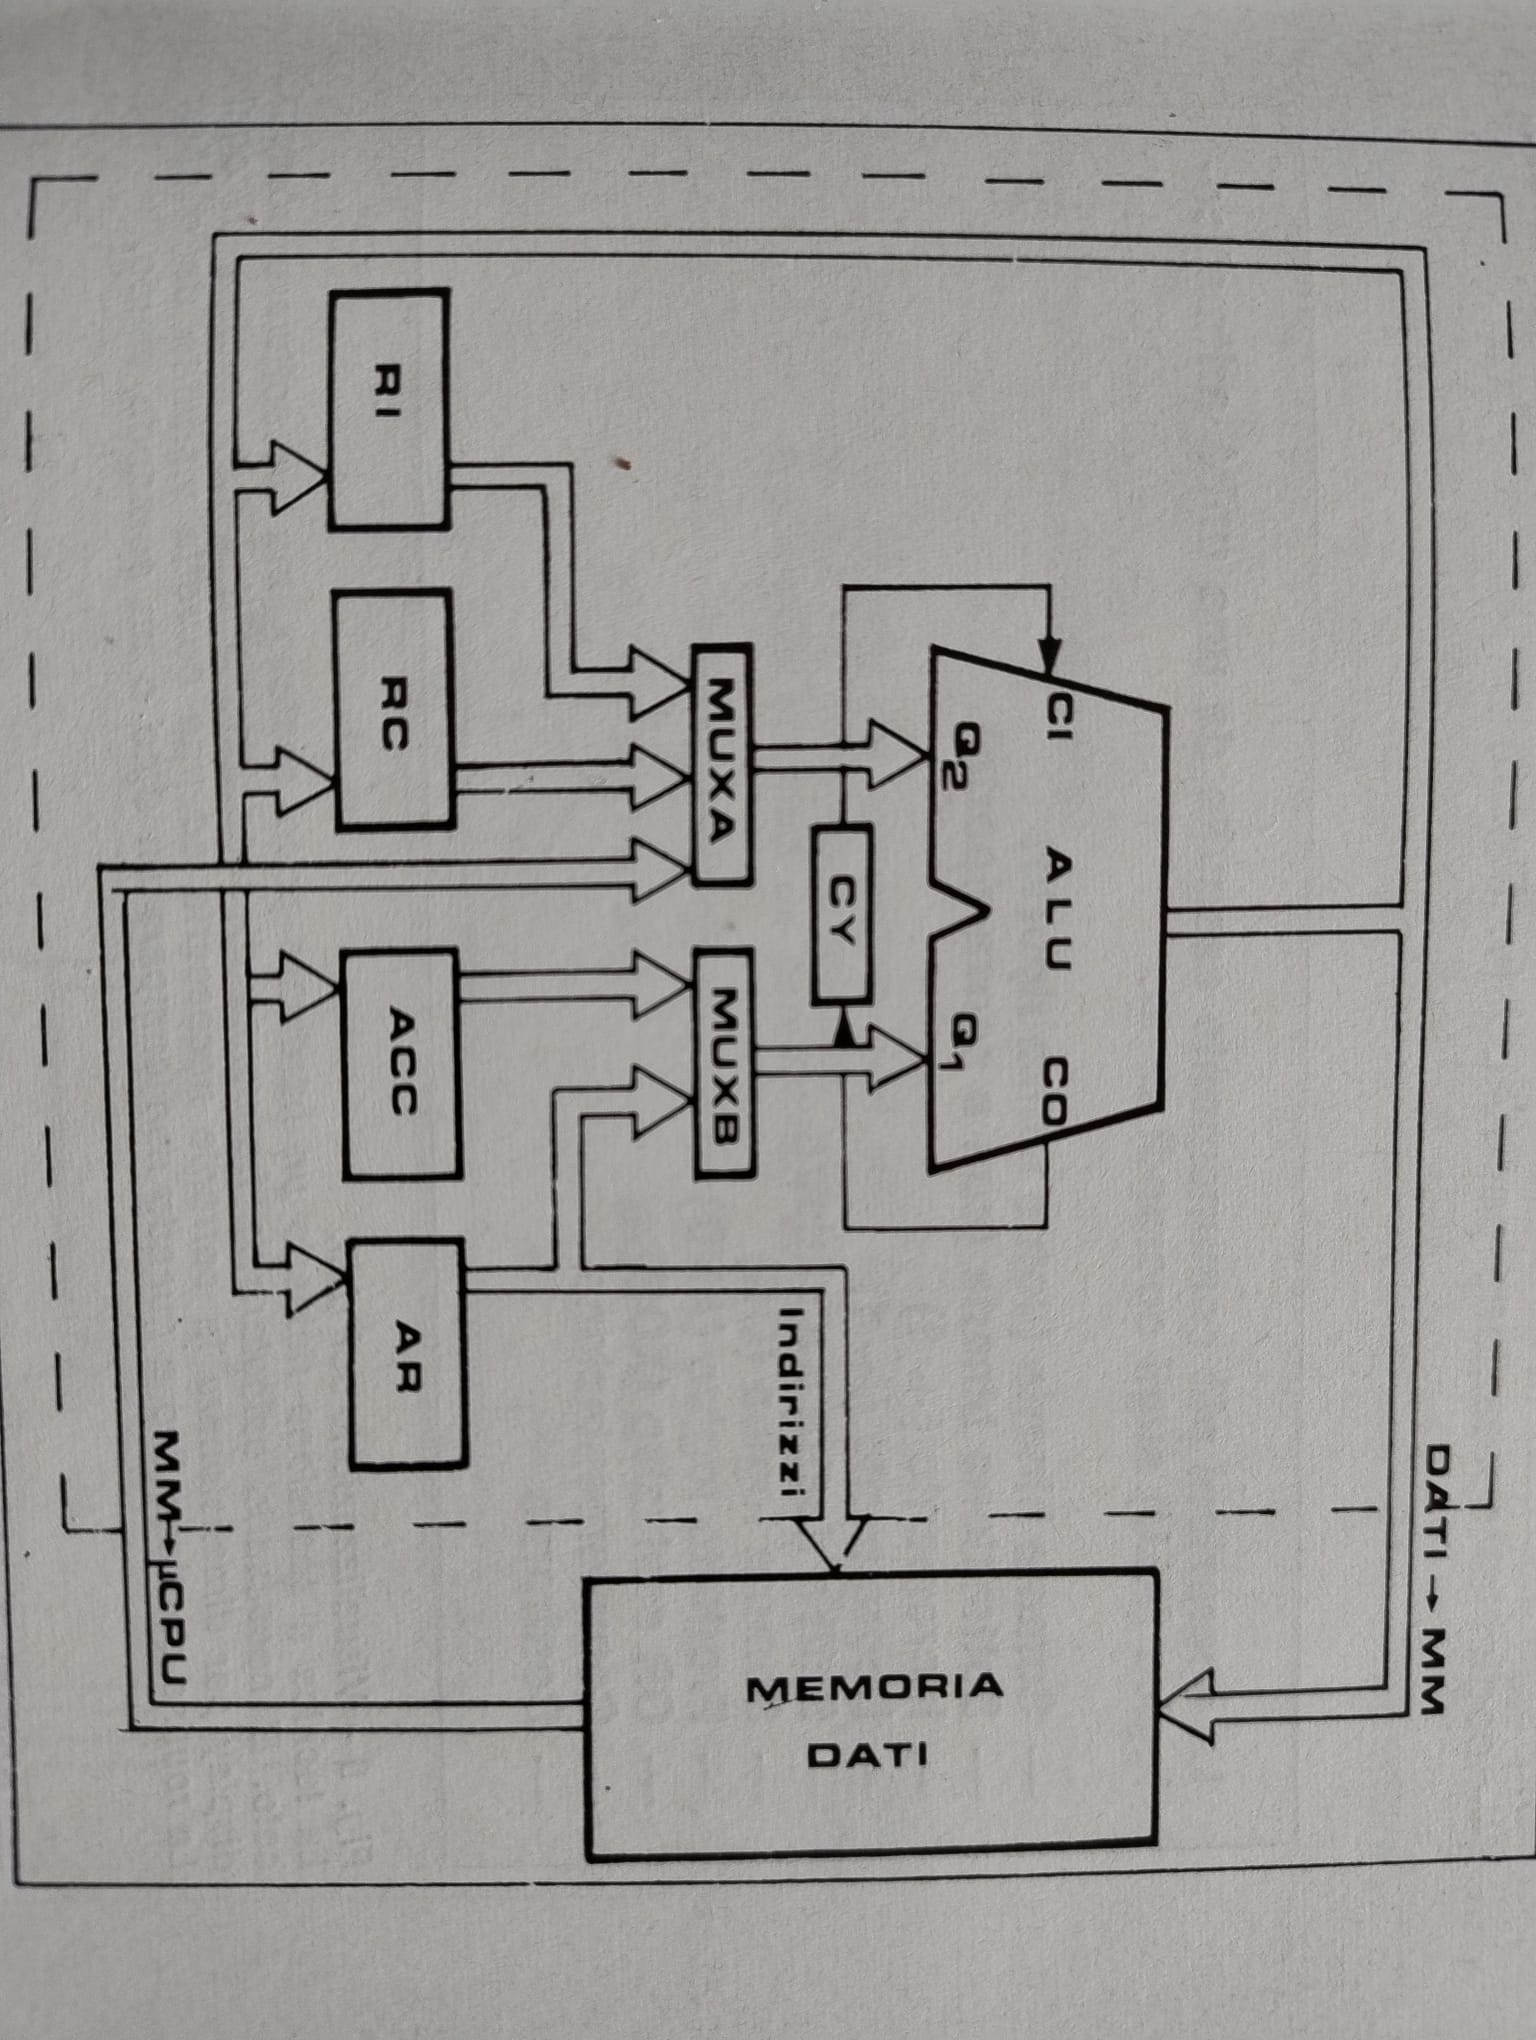
\includegraphics[width=0.6\textwidth]{schema.jpeg}
    \caption{Schema dell'architettura con i registri e l'ALU.}
    \label{fig:schema}
\end{figure}

Verranno analizzate le singole fasi dell'algoritmo, mettendo in luce:
\begin{itemize}
    \item Il ruolo di ciascun registro;
    \item L'inizializzazione dei valori di \texttt{carry} e degli indici;
    \item Il ciclo di lettura dei bit, la somma e l'immagazzinamento del risultato parziale;
    \item Il controllo dell'indice e la gestione del \texttt{carry} finale.
\end{itemize}

Inoltre, metteremo in relazione questo processo con alcuni concetti fondamentali di teoria degli automi, come l'automa a stati finiti (FSM), l'automa a pila (PDA) e la Macchina di Turing (MdT). Tali riferimenti sono utili a comprendere la natura sequenziale e a stati dell'algoritmo, nonché l'idea di come si possa estendere a meccanismi di calcolo più potenti (ad esempio, se volessimo gestire un numero di bit potenzialmente molto grande).

\section{Descrizione dell'Architettura}
Lo schema a blocchi dell'architettura proposta mostra diversi registri e un'ALU (Arithmetic Logic Unit). I componenti principali sono:
\begin{itemize}
    \item \textbf{AR (Address Register)}: Registro che contiene l'indirizzo di memoria corrente da cui leggere o in cui scrivere.
    \item \textbf{RI (Registro Indice)}: Registro che tiene traccia dell'indice corrente, utile per iterare sui bit dei due operandi.
    \item \textbf{RC (Registro Conteggio)}: Registro che contiene il numero di bit totali da sommare (o il numero di cicli da eseguire).
    \item \textbf{ACC (Accumulator)}: Registro accumulatore in cui si depositano i dati temporanei e i risultati intermedi di calcolo.
    \item \textbf{CY (Carry)}: Flip-flop o registro dedicato a immagazzinare il riporto (\textit{carry}) risultante dall'operazione di somma.
    \item \textbf{ALU}: L'unità aritmetico-logica che, in base ai segnali di controllo, esegue l'operazione di addizione (o altre operazioni aritmetico-logiche).
\end{itemize}

La memoria dati è organizzata in celle, ciascuna delle quali può contenere un singolo bit dell'operando (o più bit, a seconda dell'implementazione). Per semplicità, supponiamo che ogni cella di memoria contenga \textbf{un singolo bit}.

Nell'architettura, vediamo come l'ALU abbia diversi ingressi provenienti da multiplexer (\texttt{MUXA} e \texttt{MUXB}), i quali selezionano quale registro o bus deve essere collegato all'ingresso dell'ALU. L'uscita dell'ALU, oltre a fornire il risultato dell'operazione, aggiorna il \texttt{carry} (\texttt{CY}).

\section{Il Diagramma di Flusso: Fasi Principali}
Il diagramma di flusso rappresenta l'algoritmo di somma passo per passo (Figura \ref{fig:algoritmo}). Di seguito, riportiamo una descrizione testuale dettagliata dei blocchi, collegandoli all'architettura mostrata in Figura \ref{fig:schema}.

\subsection{Caricamento e Inizializzazione}
\begin{enumerate}
    \item \textbf{Carica la costante \texttt{S} in \texttt{RC}}: la costante \texttt{S} rappresenta il numero di bit dei due operandi (supponendo siano lunghi uguale). In \texttt{RC} memorizziamo tale valore, che useremo per sapere quante iterazioni fare.
    \item \textbf{Azzera il \texttt{carry}}: poniamo a zero il registro \texttt{CY}, in quanto inizialmente non abbiamo nessun riporto in ingresso.
    \item \textbf{Azzera il registro \texttt{RI}}: \texttt{RI} viene impostato a 0 per indicare che non abbiamo ancora elaborato alcun bit.
    \item \textbf{Punta \texttt{AR} al 1\textsuperscript{o} operando}: il registro \texttt{AR} (Address Register) viene impostato all'indirizzo di memoria dove inizia il primo operando.
\end{enumerate}

\subsection{Lettura del Primo Operando}
\begin{enumerate}
    \item \textbf{Trasferisci il bit in \texttt{ACC}}: leggiamo dalla memoria (all'indirizzo puntato da \texttt{AR}) il bit corrente del primo operando e lo carichiamo nell'accumulatore \texttt{ACC}.
\end{enumerate}

\subsection{Lettura del Secondo Operando}
\begin{enumerate}
    \item \textbf{Punta \texttt{AR} al 2\textsuperscript{o} operando}: aggiorniamo \texttt{AR} in modo che punti all'indirizzo di memoria dove è memorizzato il bit corrispondente del secondo operando.
    \item \textbf{Somma in \texttt{ALU} con \texttt{CY}}: l'ALU somma il contenuto di \texttt{ACC}, il bit del secondo operando (letto in memoria) e il \texttt{carry} \texttt{CY}. Il risultato (bit di somma) viene scritto in \texttt{ACC} e \texttt{CY} viene aggiornato se c'è un riporto (cioè se la somma dei bit è 2 o 3 in decimale, corrispondente a 10 o 11 in binario).
\end{enumerate}

\subsection{Memorizzazione del Risultato Parziale}
\begin{enumerate}
    \item \textbf{Punta \texttt{AR} alla zona di memoria per il risultato}: impostiamo \texttt{AR} sull'indirizzo di memoria dove vogliamo salvare il bit di risultato.
    \item \textbf{Trasferisci il risultato in memoria}: il contenuto di \texttt{ACC} (bit di risultato) viene scritto nella cella di memoria puntata da \texttt{AR}.
\end{enumerate}

\subsection{Aggiornamento Indice e Verifica di Fine}
\begin{enumerate}
    \item \textbf{Incrementa \texttt{RI}}: il registro indice \texttt{RI} viene incrementato di 1, perché abbiamo elaborato un bit.
    \item \textbf{Confronta \texttt{RI} con \texttt{RC}}: se \texttt{RI} è uguale a \texttt{RC}, significa che abbiamo terminato di sommare tutti i bit previsti. Altrimenti, se \texttt{RI} < \texttt{RC}, ripetiamo il ciclo di somma sul bit successivo.
\end{enumerate}

\subsection{Gestione del \texttt{carry} Finale}
Se, dopo aver elaborato l'ultimo bit, \texttt{CY} risulta ancora a 1, significa che c'è un riporto finale. In tal caso, si deve:
\begin{itemize}
    \item Allocare una cella di memoria aggiuntiva per questo bit di riporto;
    \item Scrivere il valore di \texttt{CY} in tale cella, in modo da ottenere la corretta somma finale (che avrà un bit in più).
\end{itemize}

\section{Analisi dell'Algoritmo come Automa a Stati Finiti}
L'algoritmo di somma può essere visto come un \textbf{automa a stati finiti} (FSM, Finite State Machine), dove ciascun blocco del diagramma di flusso corrisponde a uno \emph{stato} o a una \emph{transizione} tra stati. 

\subsection{Stati e Transizioni}
\begin{itemize}
    \item \textbf{Stato di inizializzazione}: l'automa si trova nello stato in cui \texttt{RC}, \texttt{RI} e \texttt{CY} vengono inizializzati. Al termine di questa fase, si passa allo stato successivo.
    \item \textbf{Stato di lettura primo operando}: si legge il bit dal primo operando, si carica in \texttt{ACC}.
    \item \textbf{Stato di lettura secondo operando e somma}: si legge il bit dal secondo operando e lo si somma con \texttt{ACC} e \texttt{CY}.
    \item \textbf{Stato di memorizzazione}: si scrive il risultato in memoria.
    \item \textbf{Stato di incremento e verifica}: si incrementa \texttt{RI}, si verifica se \texttt{RI} = \texttt{RC}.
\end{itemize}

Ciascuno stato ha delle \textit{condizioni di uscita} che determinano se passare allo stato successivo o terminare (in caso di \texttt{RI} = \texttt{RC} e gestione dell'eventuale \texttt{carry} finale).

\subsection{Osservazioni}
Questo modello di calcolo è sequenziale e \textit{limitato} dal numero di stati previsti. Un FSM puro, infatti, ha un numero finito di stati e non dispone di memoria ausiliaria arbitraria. Qui, la memoria per la gestione dei dati è esterna (la RAM), ma la sequenza di controllo dell'algoritmo si può comunque mappare su un insieme finito di stati.

\section{Collegamento con Automi a Pila e Macchina di Turing}
\subsection{Automa a Pila (PDA)}
Un \textbf{automa a pila} è un automa a stati finiti dotato di una memoria a pila. Se consideriamo la \textit{pila} come un meccanismo per gestire il \texttt{carry} o per immagazzinare i bit dei risultati intermedi, potremmo \emph{estendere} l'algoritmo in modo da supportare, ad esempio, la somma di numeri rappresentati in modo più complesso (o con struttura ricorsiva). Tuttavia, per l'algoritmo di somma di base, la memoria a pila non è strettamente necessaria: la gestione del \texttt{carry} avviene tramite un singolo bit dedicato e la memorizzazione dei bit avviene in RAM.

\subsection{Macchina di Turing (MdT)}
Una \textbf{Macchina di Turing} è un modello di calcolo più potente, che può simulare qualsiasi algoritmo. L'algoritmo di somma di due numeri può essere realizzato facilmente da una MdT, la quale sposterebbe la testina su un nastro di memoria, leggendo e scrivendo bit, eventualmente tenendo traccia del \texttt{carry} in uno stato interno. 

In un certo senso, l'architettura di un calcolatore reale (con registri, ALU, memoria, bus, ecc.) può essere vista come un'implementazione pratica di una Macchina di Turing limitata dalla dimensione finita della memoria. Il nostro algoritmo di somma è un \textit{caso particolare} di operazione aritmetica, ma dimostra bene la natura sequenziale, a stati e basata sulla memoria, tipica di ogni calcolatore.

\section{Dettagli Implementativi}
\subsection{Modalità di Indirizzamento}
Nell'architettura mostrata, il registro \texttt{AR} punta di volta in volta a:
\begin{enumerate}
    \item Celle del primo operando;
    \item Celle del secondo operando;
    \item Celle del risultato.
\end{enumerate}
Ogni volta che passiamo dal primo al secondo operando, cambiamo il valore di \texttt{AR}. Analogamente, quando vogliamo scrivere il risultato, impostiamo \texttt{AR} sull'area di memoria destinata al risultato.

\subsection{Ruolo del Registro Indice \texttt{RI}}
\texttt{RI} funge da contatore del numero di bit elaborati. In molte architetture reali, \texttt{RI} potrebbe essere incrementato automaticamente dopo ogni accesso in memoria (\emph{auto-increment}), oppure potremmo avere istruzioni dedicate per incrementare \texttt{RI}. In ogni caso, \texttt{RI} viene confrontato con \texttt{RC} (che rappresenta il numero totale di bit) per stabilire il \emph{punto di uscita} dal ciclo di somma.

\subsection{Gestione del \texttt{carry}}
Il \texttt{carry} (\texttt{CY}) è un singolo bit che può assumere valore 0 o 1. Nelle architetture binarie, ciò accade quando la somma dei bit in ingresso supera la capacità di 1 bit. In particolare:
\begin{itemize}
    \item 0 + 0 + \texttt{carry}(0) = 0 (nessun riporto)
    \item 1 + 0 + \texttt{carry}(0) = 1 (nessun riporto)
    \item 1 + 1 + \texttt{carry}(0) = 0 (con riporto = 1)
    \item 1 + 1 + \texttt{carry}(1) = 1 (con riporto = 1)
\end{itemize}
Se stiamo lavorando in binario, questa logica è integrata nell'ALU. Il \texttt{carry} aggiornato viene poi conservato per l'iterazione successiva.

\section{Esempio di Funzionamento in Binario}
Supponiamo di voler sommare i numeri (in binario) \texttt{1100} (che corrisponde a 12 in decimale) e \texttt{1011} (che corrisponde a 11 in decimale). Entrambi hanno 4 bit, quindi \texttt{S} = 4. L'ordine di elaborazione dei bit, nel caso classico, parte dal \textit{meno significativo} (a destra) verso il \textit{più significativo} (a sinistra). Pertanto, i bit saranno gestiti nel seguente ordine:

\begin{center}
\begin{tabular}{c|c|c|c|c}
\textbf{Bit Index} & \textbf{3 (MSB)} & \textbf{2} & \textbf{1} & \textbf{0 (LSB)} \\
\hline
\textbf{1100 (A)} & 1 & 1 & 0 & 0 \\
\textbf{1011 (B)} & 1 & 0 & 1 & 1 \\
\end{tabular}
\end{center}

Vediamo passo passo:

\subsection*{Bit LSB (Indice 0)}
\begin{enumerate}
    \item \texttt{RI} $\leftarrow$ 0, \texttt{CY} $\leftarrow$ 0.
    \item Leggiamo bit 0 di A: 0. Carichiamo in \texttt{ACC}.
    \item Leggiamo bit 0 di B: 1. Sommiamo \texttt{ACC} (0), B (1) e \texttt{CY} (0) = 1, \texttt{CY} = 0.
    \item Scriviamo 1 in memoria come bit 0 del risultato.
    \item \texttt{RI} $\leftarrow$ 1. \texttt{RI} < \texttt{RC} (1 < 4) $\rightarrow$ continuiamo.
\end{enumerate}

\subsection*{Bit di indice 1}
\begin{enumerate}
    \item Leggiamo bit 1 di A: 0. \texttt{ACC} = 0.
    \item Leggiamo bit 1 di B: 1. Sommiamo \texttt{ACC} (0), B (1) e \texttt{CY} (0) = 1, \texttt{CY} = 0.
    \item Scriviamo 1 in memoria come bit 1 del risultato.
    \item \texttt{RI} $\leftarrow$ 2. \texttt{RI} < \texttt{RC} (2 < 4) $\rightarrow$ continuiamo.
\end{enumerate}

\subsection*{Bit di indice 2}
\begin{enumerate}
    \item Leggiamo bit 2 di A: 1. \texttt{ACC} = 1.
    \item Leggiamo bit 2 di B: 0. Sommiamo \texttt{ACC} (1), B (0) e \texttt{CY} (0) = 1, \texttt{CY} = 0.
    \item Scriviamo 1 in memoria come bit 2 del risultato.
    \item \texttt{RI} $\leftarrow$ 3. \texttt{RI} < \texttt{RC} (3 < 4) $\rightarrow$ continuiamo.
\end{enumerate}

\subsection*{Bit di indice 3 (MSB)}
\begin{enumerate}
    \item Leggiamo bit 3 di A: 1. \texttt{ACC} = 1.
    \item Leggiamo bit 3 di B: 1. Sommiamo \texttt{ACC} (1), B (1) e \texttt{CY} (0). \\
    La somma binaria di 1 + 1 = 10 (in binario), quindi il risultato nel \texttt{ACC} sarà 0, e \texttt{CY} = 1.
    \item Scriviamo 0 in memoria come bit 3 del risultato.
    \item \texttt{RI} $\leftarrow$ 4. Ora \texttt{RI} = \texttt{RC} (4 = 4).
\end{enumerate}

A questo punto, abbiamo \texttt{CY} = 1, il che indica un riporto \emph{finale}. Poiché \texttt{RI} = \texttt{RC}, controlliamo se \texttt{CY} = 1. Se sì, scriviamo questo bit in una nuova cella di memoria (bit di indice 4 del risultato).

\subsection*{Bit di riporto finale}
\begin{enumerate}
    \item Scriviamo \texttt{CY} (1) nella cella di memoria successiva (indice 4).
\end{enumerate}

\noindent
Ricostruendo il risultato dal bit meno significativo a quello più significativo, otteniamo:
\[
\text{Risultato} = 
\underbrace{1}_{\text{Carry finale}}
\underbrace{0}_{\text{bit 3}}
\underbrace{1}_{\text{bit 2}}
\underbrace{1}_{\text{bit 1}}
\underbrace{1}_{\text{bit 0}}
= 10111_2
\]
che in decimale corrisponde a 23 (infatti 12 + 11 = 23).

\section{Conclusioni}
L'algoritmo di somma descritto è un tipico esempio di come, all'interno di un calcolatore, si possa implementare un'operazione aritmetica di base in \textbf{binario}. L'uso di registri specifici (\texttt{AR}, \texttt{RI}, \texttt{RC}, \texttt{ACC}, \texttt{CY}) e la gestione sequenziale dell'accesso alla memoria mostrano la natura a \textit{stati finiti} del \textit{controllo} del processore, mentre la memoria dati fornisce lo spazio per operandi e risultati. 

Collegando il tutto alla teoria degli automi, notiamo che:
\begin{itemize}
    \item Come FSM, l'algoritmo è descritto da un numero finito di stati e transizioni (inizializzazione, lettura, somma, scrittura, incremento indice, ecc.).
    \item Non è strettamente necessario un automa a pila (PDA) per realizzare questa operazione, sebbene una pila possa essere introdotta per estensioni più complesse (ad esempio, per gestire forme di notazione più articolate).
    \item Qualsiasi architettura di calcolatore, nella sua interezza, può essere considerata una Macchina di Turing finita (a causa dei limiti di memoria fisica), ma \textit{equivalente} a una MdT \emph{ideale} dal punto di vista computazionale, almeno finché non si esauriscono le risorse di memoria.
\end{itemize}

L'implementazione in linguaggio macchina (o microcodice) di questo algoritmo segue fedelmente il diagramma di flusso. Ciascuna istruzione \texttt{move}, \texttt{add}, \texttt{store} corrisponde a uno dei blocchi indicati. Il \texttt{carry} viene gestito da segnali di controllo interni all'ALU. Infine, l'architettura può essere generalizzata per altre operazioni (sottrazione, moltiplicazione, divisione) adottando schemi simili e integrando i necessari segnali di controllo nell'ALU.

%#######################

\chapter{Collaborazione Creativi e Tecnici: Un Progetto Interdisciplinare}

\section{Introduzione al Progetto}
L'obiettivo di questo progetto \`e stimolare la collaborazione tra studenti con competenze creative e tecniche, unendo il mondo artistico a quello dell'ingegneria. Il punto di partenza \`e un semplice gioco implementato con Arduino, che utilizza pulsanti e LED per creare una sequenza di stati basati su un automa a stati finiti. 

Il progetto si evolve trasformando questo prototipo in un'esperienza arricchita, dove ogni squadra \`e chiamata a contribuire in base alle proprie capacit\`a:
\begin{itemize}
    \item Il \textbf{Team Creativo} immagina come rendere il gioco pi\`u accessibile, originale e coinvolgente, progettando controller, decorazioni e contesti narrativi.
    \item Il \textbf{Team Tecnico} traduce queste idee in soluzioni pratiche, realizzando i controller e migliorando il sistema Arduino per implementare le modifiche richieste.
\end{itemize}

La sfida \`e creare un gioco che sia divertente, esteticamente accattivante e tecnicamente funzionale, favorendo al contempo la comunicazione e la collaborazione tra i due team.

\section{Guida per il Team Creativo}
I creativi hanno il compito di trasformare il progetto da un semplice prototipo tecnico a un'esperienza visiva e interattiva unica. Per fare ci\`o, possono seguire questi passaggi:

\subsection{Brainstorming delle Idee}
Iniziate immaginando come migliorare il gioco:
\begin{itemize}
    \item \textbf{Controller originale}: Pensate a un design che i giocatori possano utilizzare facilmente, come:
    \begin{itemize}
        \item Controller da tenere in mano con una forma ergonomica e colori vivaci.
        \item Pedali per controllare il gioco con i piedi.
        \item Oggetti interattivi che si attivano toccandoli o muovendoli.
    \end{itemize}
    \item \textbf{Elementi visivi}: Create decorazioni che rappresentino la storia del gioco, come un'ambientazione spaziale o un cruscotto di comando futuristico.
    \item \textbf{Esperienza sociale}: Progettate il gioco in modo che i giocatori interagiscano fisicamente o socialmente tra loro.
\end{itemize}

\subsection{Creazione di Schizzi e Prototipi}
Dopo aver definito le idee, rappresentatele visivamente:
\begin{itemize}
    \item \textbf{Disegni}: Usate carta, matite colorate o software come Canva o TinkerCAD per creare rappresentazioni delle vostre idee.
    \item \textbf{Prototipi fisici}: Costruite modelli con materiali semplici come carta, cartone, carta pesta o plastica riciclata.
    \item \textbf{Moodboard}: Realizzate un collage di immagini che trasmetta l'estetica e l'atmosfera del progetto.
\end{itemize}

\subsection{Presentazione delle Idee}
Organizzate una presentazione per condividere le vostre idee con il Team Tecnico. Assicuratevi di includere:
\begin{itemize}
    \item Schizzi o prototipi.
    \item Una spiegazione chiara delle funzionalit\`a e dell'estetica proposte.
    \item Eventuali sfide tecniche che immaginate e come potrebbero essere affrontate.
\end{itemize}

\begin{figure}[ht!]
    \centering
    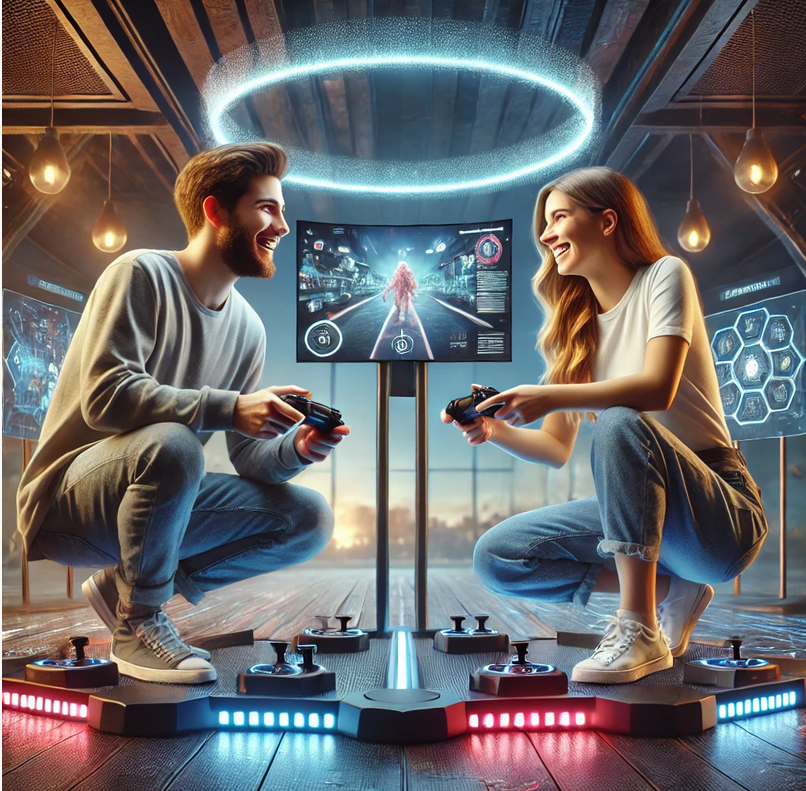
\includegraphics[width=0.6\textwidth]{creativi.png}
    \caption{Un esempio di creativit\`a nel design del gioco.}
    \label{fig:creativi}
\end{figure}

\section{Guida per il Team Tecnico}
I tecnici hanno il compito di implementare le idee del Team Creativo utilizzando soluzioni pratiche ed efficaci. Questo richiede la conoscenza di alcuni componenti chiave e la capacit\`a di integrarli nel sistema Arduino.

\subsection{Componenti Principali}
\begin{itemize}
    \item \textbf{Sensori}: Dispositivi che convertono un fenomeno fisico (pressione, movimento, tocco) in segnali elettronici. Esempi:
    \begin{itemize}
        \item \textbf{Sensore di pressione (FSR)}: Rileva la forza esercitata su una superficie, ideale per pedali.
        \item \textbf{Sensore touch capacitivo}: Rileva il tocco su una superficie conduttiva, utile per controller tattili.
    \end{itemize}
    \item \textbf{Accelerometri}: Dispositivi che misurano l'accelerazione o il movimento. Possono essere usati per controlli basati sul movimento del corpo (ad esempio, inclinazione o rotazione).
    \item \textbf{LED RGB}: LED che possono emettere una combinazione di colori. Utilizzati per creare effetti visivi accattivanti.
    \item \textbf{Pulsanti arcade}: Pulsanti robusti e colorati, ideali per controller manuali.
\end{itemize}

\subsection{Realizzazione Tecnica}
\begin{itemize}
    \item \textbf{Prototipazione su breadboard}: Utilizzate una breadboard per testare i componenti prima di realizzare un circuito definitivo.
    \item \textbf{Saldatura e cablaggio}: Dopo i test, assemblate i componenti su un circuito stampato o un supporto stabile.
    \item \textbf{Programmazione}: Scrivete il codice Arduino per gestire i nuovi input e output, implementando le modifiche richieste.
\end{itemize}

\subsection{Debug e Ottimizzazione}
Assicuratevi che il sistema funzioni correttamente:
\begin{itemize}
    \item Testate ogni componente individualmente prima di integrarli.
    \item Monitorate il comportamento del sistema utilizzando la comunicazione seriale di Arduino.
    \item Collaborate con il Team Creativo per apportare modifiche in base al feedback.
\end{itemize}

\begin{figure}[ht!]
    \centering
    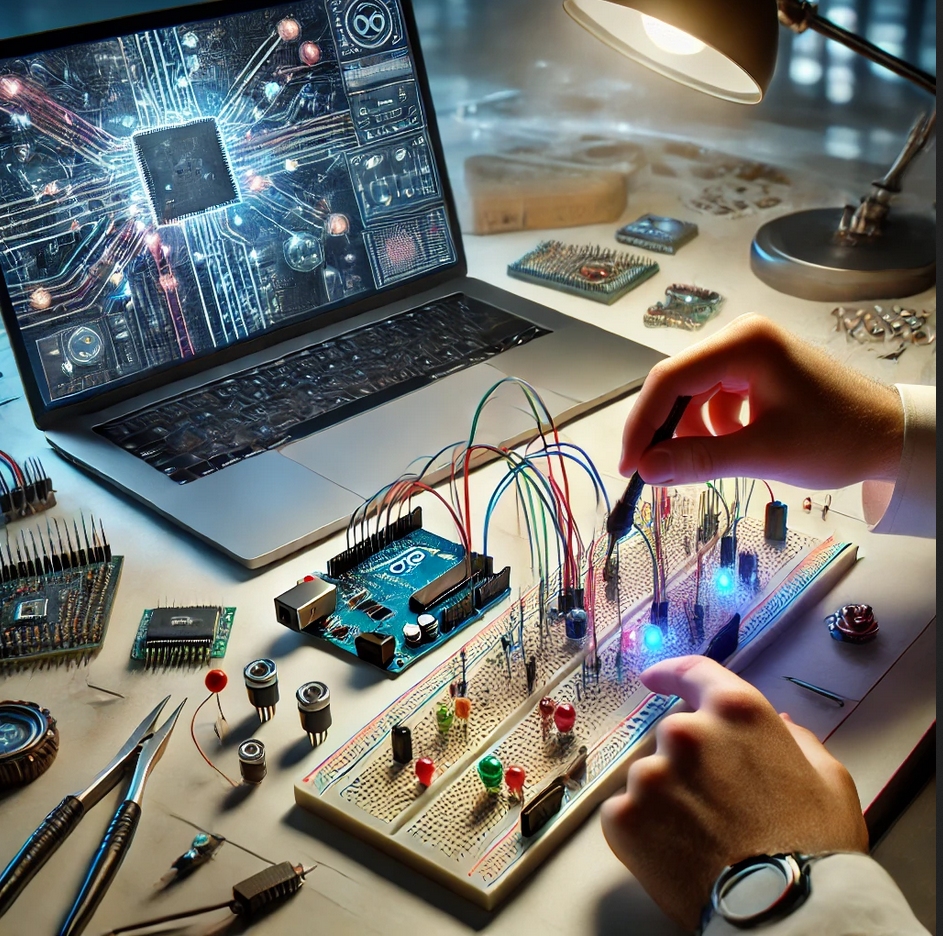
\includegraphics[width=0.6\textwidth]{tecnici.png}
    \caption{Un esempio di lavoro tecnico per implementare le idee del progetto.}
    \label{fig:tecnici}
\end{figure}

\subsection{Presentazione del Progetto}
Documentate il processo tecnico e preparate una presentazione che mostri:
\begin{itemize}
    \item I componenti scelti e come sono stati integrati.
    \item Le sfide incontrate e come sono state risolte.
    \item Il risultato finale e come soddisfa i requisiti del Team Creativo.
\end{itemize}

\section{Progettazione e Creazione del Package}
\subsection{Design del Package}
Per racchiudere e proteggere il sistema, il package deve essere progettato considerando sia l'estetica che la funzionalit\`a. Ecco alcune linee guida:
\begin{itemize}
    \item \textbf{Materiali}: Scegliete materiali leggeri ma resistenti come plastica riciclata, legno o acrilico.
    \item \textbf{Forma}: Il design deve essere ergonomico e funzionale, consentendo ai giocatori di interagire comodamente con il sistema.
    \item \textbf{Decorazioni}: Collaborate con il Team Creativo per integrare decorazioni che riflettano il tema del gioco.
\end{itemize}

\subsection{Processo di Costruzione}
\begin{itemize}
    \item \textbf{Prototipazione}: Costruite un modello in scala con materiali economici come cartone o foamboard per testare il design.
    \item \textbf{Taglio e Assemblaggio}: Utilizzate strumenti come taglierine laser o stampanti 3D per realizzare il package definitivo.
    \item \textbf{Integrazione dei Componenti}: Alloggiate saldamente i componenti elettronici nel package, assicurandovi che siano facilmente accessibili per manutenzione o aggiornamenti.
\end{itemize}

\subsection{Test del Package}
\begin{itemize}
    \item Verificate che il package protegga adeguatamente i componenti elettronici.
    \item Assicuratevi che il package sia comodo da usare per i giocatori.
    \item Fate test di durabilit\`a per garantire che il package resista a un uso prolungato.
\end{itemize}

\section{Componenti del Gioco e il loro Funzionamento}

In questa sezione descriviamo i principali componenti elettronici utilizzati per il gioco e approfondiamo i concetti fisici fondamentali che ne regolano il funzionamento.

\subsection{Legge di Ohm e Legge di Joule}
Prima di analizzare i componenti, è essenziale comprendere due leggi fondamentali dell'elettricità:
\begin{enumerate}
    \item \textbf{Legge di Ohm:} Descrive la relazione tra tensione (\(V\)), corrente (\(I\)) e resistenza (\(R\)):
    \[
    V = I \cdot R
    \]
    \item \textbf{Legge di Joule:} Descrive la potenza dissipata sotto forma di calore in un resistore:
    \[
    P = I^2 \cdot R
    \]
    dove \(P\) è la potenza (in watt), \(I\) la corrente (in ampere) e \(R\) la resistenza (in ohm).
\end{enumerate}

Queste leggi sono fondamentali per dimensionare correttamente le resistenze e garantire che i LED non vengano danneggiati da una corrente eccessiva.

---

\subsection{LED e Semiconduttori}
\textbf{Principio di Funzionamento:} I LED (\textit{Light Emitting Diodes}) sono dispositivi semiconduttori che emettono luce quando attraversati da corrente elettrica in polarizzazione diretta.

\textbf{Cosa sono i semiconduttori?}
\begin{itemize}
    \item I semiconduttori (es. silicio e arsenico di gallio) hanno una conducibilità intermedia tra conduttori e isolanti.
    \item La loro conducibilità può essere modificata aggiungendo impurità (\textit{drogaggio}), creando zone di tipo \(p\) (ricche di lacune) e di tipo \(n\) (ricche di elettroni).
\end{itemize}

\textbf{Emissione di luce senza effetto Joule:}
Quando un elettrone si ricombina con una lacuna in una giunzione \(p\)-\(n\), rilascia energia sotto forma di un fotone (luce). Questa energia è determinata dalla banda proibita (\(E_g\)) del materiale semiconduttore:
\[
E = h \cdot f
\]
dove:
\begin{itemize}
    \item \(E\) è l'energia del fotone.
    \item \(h\) è la costante di Planck (\(6.63 \cdot 10^{-34} \, \text{J·s}\)).
    \item \(f\) è la frequenza della luce emessa.
\end{itemize}

A differenza delle resistenze, l'emissione di luce nei LED non avviene tramite l'effetto Joule, ma tramite transizioni elettroniche, rendendoli efficienti dal punto di vista energetico.

---

\subsection{Altri Componenti e Collegamenti}
\subsubsection{Resistenze}
\textbf{Calcolo della resistenza per un LED:}
Per evitare sovracorrenti nei LED, è necessario calcolare il valore della resistenza:
\[
R = \frac{V_{\text{alimentazione}} - V_{\text{LED}}}{I_{\text{LED}}}
\]
dove:
\begin{itemize}
    \item \(V_{\text{alimentazione}}\) è la tensione fornita da Arduino (es. 5V).
    \item \(V_{\text{LED}}\) è la caduta di tensione tipica del LED (es. 2V per un LED rosso).
    \item \(I_{\text{LED}}\) è la corrente desiderata (tipicamente 20mA).
\end{itemize}

---

\subsubsection{Bottoni e Interruttori}
\textbf{Funzionamento:} I bottoni momentanei chiudono il circuito solo quando premuti. Sono utilizzati come input digitali per Arduino.

\textbf{Problema dei segnali fluttuanti:} Senza una resistenza di pull-up o pull-down, il segnale del bottone può essere instabile, generando falsi input.

\textbf{Soluzione:} Usa una resistenza di pull-up (connessa a \(V_{\text{cc}}\)) o pull-down (connessa a \(GND\)) per stabilizzare il segnale:
\[
R_{\text{pull-up/pull-down}} \approx 10 \, \text{k}\Omega
\]

---

\subsubsection{Arduino Uno}
\textbf{Specifiche principali:}
\begin{itemize}
    \item Microcontrollore ATmega328.
    \item Tensione operativa: 5V.
    \item Ingressi digitali e analogici per il controllo di sensori e attuatori.
\end{itemize}

\begin{figure}[H]
    \centering
    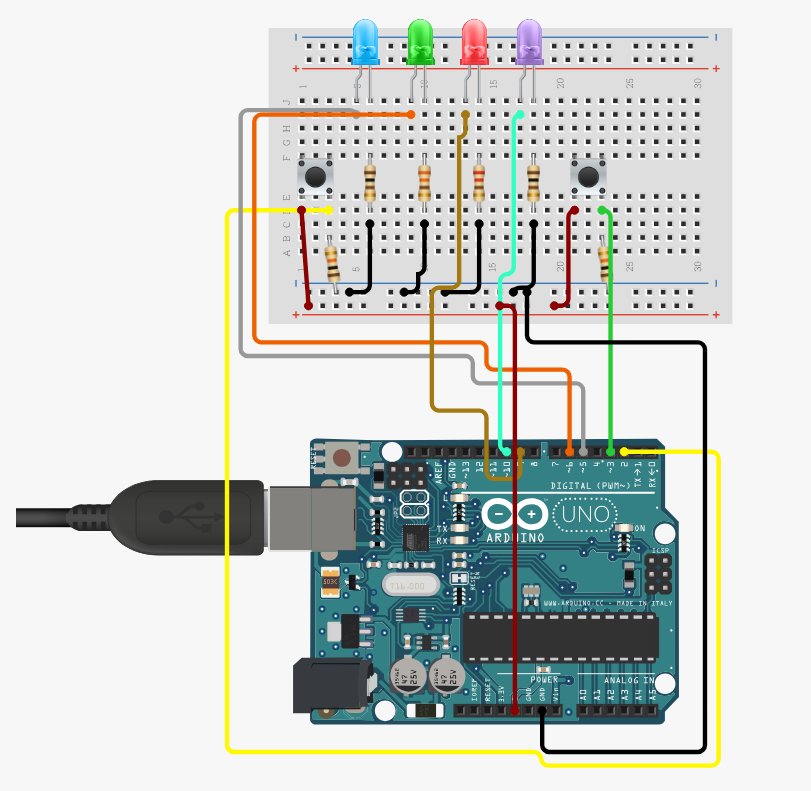
\includegraphics[width=0.6\textwidth]{arduino.png}
    \caption{Diagramma dei collegamenti}
    \label{fig:full_adder}
\end{figure}

\chapter{Introduzione a Python e Simulazione del Gioco dei 4 Colori}

\section{Introduzione a Python}
Python è un linguaggio di programmazione ad alto livello, ampiamente utilizzato per la sua sintassi semplice e leggibilità. È ideale per imparare i concetti base della programmazione e per creare applicazioni pratiche.

\subsection{La Sintassi Base di Python}
In Python, il codice si organizza in blocchi identificati dall'indentazione. Ecco alcune strutture base:

\subsubsection*{Stampa e Input}
\begin{lstlisting}[language=Python, caption={Esempio di stampa e input}]
print("Ciao, mondo!")  # Stampa un messaggio a schermo
nome = input("Come ti chiami? ")  # Chiede un input all'utente
print("Benvenuto, " + nome + "!")
\end{lstlisting}

\subsubsection*{Condizioni e Cicli}
\begin{lstlisting}[language=Python, caption={Esempio di condizioni e cicli}]
# Esempio di condizione
numero = int(input("Inserisci un numero: "))
if numero > 0:
    print("Il numero è positivo.")
else:
    print("Il numero è zero o negativo.")

# Esempio di ciclo
for i in range(5):  # Ripete per i valori da 0 a 4
    print("Iterazione:", i)
\end{lstlisting}

\subsubsection*{Funzioni}
\begin{lstlisting}[language=Python, caption={Esempio di funzione}]
# Una funzione che calcola il quadrato di un numero
def quadrato(x):
    return x * x

risultato = quadrato(4)
print("Il quadrato di 4 è:", risultato)
\end{lstlisting}

\section{Python e gli Automi}
Un programma in Python può essere considerato equivalente a un automa perché entrambi seguono regole precise di transizione da uno stato all'altro basandosi sugli input ricevuti.

\subsection{Esempio di Automa in Python}
Un automa a stati finiti per il gioco dei 4 colori può essere rappresentato in Python come segue:
\begin{lstlisting}[language=Python, caption={Esempio di automa a stati finiti in Python}]
# Definizione degli stati
stati = ["R", "G", "B", "W"]
stato_corrente = "R"

# Funzione per la transizione
def transizione(giocatore):
    global stato_corrente
    if stato_corrente == "R":
        stato_corrente = "G" if giocatore == 1 else "B"
    elif stato_corrente == "G":
        stato_corrente = "B" if giocatore == 1 else "R"
    elif stato_corrente == "B":
        stato_corrente = "W"
    elif stato_corrente == "W":
        stato_corrente = "R" if giocatore == 1 else "G"

# Simulazione
print("Stato iniziale:", stato_corrente)
transizione(1)  # Giocatore 1 preme il tasto
print("Stato dopo Giocatore 1:", stato_corrente)
transizione(2)  # Giocatore 2 preme il tasto
print("Stato dopo Giocatore 2:", stato_corrente)
\end{lstlisting}

\section{Simulazione del Gioco dei 4 Colori}
Portiamo il nostro gioco completo in Python. La sequenza di gioco è la seguente:
\begin{enumerate}
    \item Il sistema genera una sequenza casuale di transizioni.
    \item Mostra la sequenza ai giocatori.
    \item I giocatori ripetono la sequenza premendo i tasti corretti.
    \item Il sistema verifica se la sequenza dei giocatori è corretta.
\end{enumerate}

\subsection{Codice Completo in Python}
\lstinputlisting[language=Python, caption={Codice Python del gioco dei 4 colori}, label={lst:gioco_python}]{gioco_4_colori.py}


\section{Conclusione}
Questa introduzione a Python mostra come il linguaggio possa essere utilizzato per simulare automi e implementare il gioco dei 4 colori. Gli studenti possono facilmente espandere il programma aggiungendo nuove funzionalità o modificando le regole del gioco.

\chapter{Prototipazione con cartapesta}
\section{Introduzione}
Nel corso del progetto, gli studenti hanno sviluppato tre diverse versioni di una console di gioco interattiva, combinando competenze artistiche e tecniche. La progettazione ha coinvolto sia l'aspetto estetico e di usabilità (curato dagli studenti dell'indirizzo artistico) sia la realizzazione elettronica e programmabile con Arduino (a cura degli studenti dell'indirizzo tecnico).

\section{Prototipi sviluppati}

\subsection{Console classica}
Questo prototipo è il più vicino ai videogiochi tradizionali, con due joystick e pulsanti colorati. Gli studenti hanno progettato e realizzato il case in cartapesta, garantendo un design ergonomico per un'interazione naturale con i controlli.

\begin{figure}[h]
    \centering
    \begin{tabular}{c c}
        \includegraphics[width=0.4\textwidth]{immagini/console_1.jpeg} &
        \includegraphics[width=0.4\textwidth]{immagini/cartapesta_1.jpeg} \\
    \end{tabular}
    \caption{Prototipo della console classica, con pulsanti e joystick separati.}
    \label{fig:console_classica}
\end{figure}

\subsection{Nuvola con bottoni integrati}
Questa versione presenta un design più astratto e giocoso, con i pulsanti incorporati direttamente nella superficie della console. Gli studenti dell'indirizzo artistico hanno creato il case in cartapesta, mentre il team tecnico ha integrato i circuiti e i pulsanti per la corretta interazione.

\begin{figure}[h]
    \centering
    \begin{tabular}{c c}
       \includegraphics[width=0.4\textwidth]{immagini/nuvola_3.jpeg} &
        \includegraphics[width=0.4\textwidth]{immagini/nuvola_4.jpeg} \\
        \includegraphics[width=0.4\textwidth]{immagini/nuvola_1.jpeg} &
        \includegraphics[width=0.4\textwidth]{immagini/nuvola_2.jpeg} \\
       
    \end{tabular}
    \caption{Prototipo "nuvola", con pulsanti integrati nel design della console.}
    \label{fig:nuvola}
\end{figure}

\subsection{Cocomero}
L'ultima versione della console richiama la forma di un cocomero, combinando elementi visivi accattivanti con la funzionalità interattiva. Gli studenti hanno lavorato sulla colorazione e sulla disposizione dei pulsanti, creando un design coinvolgente.

\begin{figure}[h]
    \centering
    \begin{tabular}{c c}
        \includegraphics[width=0.4\textwidth]{immagini/cocomero_1.jpeg} &
        \includegraphics[width=0.4\textwidth]{immagini/cartapesta_2.jpeg} \\
    \end{tabular}
    \caption{Prototipo "cocomero", un mix tra estetica e funzionalità di gioco.}
    \label{fig:cocomero}
\end{figure}

\section{Processo di realizzazione}
Il lavoro si è articolato in diverse fasi:
\begin{itemize}
    \item \textbf{Progettazione}: gli studenti hanno ideato il design e la disposizione dei pulsanti.
    \item \textbf{Costruzione in cartapesta}: sono stati realizzati i case con materiali modellabili e decorati a mano.
    \item \textbf{Integrazione hardware}: i circuiti con Arduino sono stati collegati ai pulsanti e ai LED, testando la funzionalità di gioco.
    \item \textbf{Programmazione}: il software su Arduino gestisce gli input degli utenti e la sequenza del gioco.
\end{itemize}

\section{Conclusioni}
Il progetto ha consentito agli studenti di esplorare la sinergia tra design e tecnologia, sviluppando competenze pratiche nella costruzione di prototipi e nella programmazione. L'approccio multidisciplinare ha favorito la collaborazione tra studenti con background differenti, valorizzando sia la creatività che la risoluzione di problemi tecnici.




\chapter{Realizzazione}

\section{Introduzione}
Nel corso del progetto, gli studenti hanno sviluppato tre diverse versioni di una console di gioco interattiva, combinando competenze artistiche e tecniche. La progettazione ha coinvolto sia l'aspetto estetico e di usabilità (curato dagli studenti dell'indirizzo artistico) sia la realizzazione elettronica e programmabile con Arduino (a cura degli studenti dell'indirizzo tecnico).

\section{Prototipi sviluppati}

\subsection{Console classica}
Questo prototipo è il più vicino ai videogiochi tradizionali, con due joystick e pulsanti colorati. Gli studenti hanno progettato e realizzato il case in cartapesta, garantendo un design ergonomico per un'interazione naturale con i controlli.

\begin{figure}[h]
    \centering
    \begin{tabular}{c c}
        \includegraphics[width=0.4\textwidth]{immagini/console_1.jpeg} &
        \includegraphics[width=0.4\textwidth]{immagini/console_3.jpeg} \\
        \includegraphics[width=0.4\textwidth]{immagini/console_4.jpeg} &
        \includegraphics[width=0.4\textwidth]{immagini/console_5.jpeg} \\
    \end{tabular}
    \caption{Prototipo della console classica, con pulsanti e joystick separati.}
    \label{fig:console_classica}
\end{figure}

\subsection{Nuvola con bottoni integrati}
Questa versione presenta un design più astratto e giocoso, con i pulsanti incorporati direttamente nella superficie della console. Gli studenti dell'indirizzo artistico hanno creato il case in cartapesta, mentre il team tecnico ha integrato i circuiti e i pulsanti per la corretta interazione.

\begin{figure}[h]
    \centering
    \begin{tabular}{c c}
        \includegraphics[width=0.4\textwidth]{immagini/nuvola_1.jpeg} &
        \includegraphics[width=0.4\textwidth]{immagini/nuvola_2.jpeg} \\
        \includegraphics[width=0.4\textwidth]{immagini/nuvola_3.jpeg} &
        \includegraphics[width=0.4\textwidth]{immagini/nuvola_4.jpeg} \\
    \end{tabular}
    \caption{Prototipo "nuvola", con pulsanti integrati nel design della console.}
    \label{fig:nuvola}
\end{figure}

\subsection{Cocomero}
L'ultima versione della console richiama la forma di un cocomero, combinando elementi visivi accattivanti con la funzionalità interattiva. Gli studenti hanno lavorato sulla colorazione e sulla disposizione dei pulsanti, creando un design coinvolgente.

\begin{figure}[h]
    \centering
    \begin{tabular}{c c}
        \includegraphics[width=0.4\textwidth]{immagini/cocomero_1.jpeg} &
        \includegraphics[width=0.4\textwidth]{immagini/cartapesta_2.jpeg} \\
        \includegraphics[width=0.4\textwidth]{immagini/cartapesta_3.jpeg} &
        \includegraphics[width=0.4\textwidth]{immagini/cartapesta_4.jpeg} \\
    \end{tabular}
    \caption{Prototipo "cocomero", un mix tra estetica e funzionalità di gioco.}
    \label{fig:cocomero}
\end{figure}

\section{Processo di realizzazione}
Il lavoro si è articolato in diverse fasi:
\begin{itemize}
    \item \textbf{Progettazione}: gli studenti hanno ideato il design e la disposizione dei pulsanti.
    \item \textbf{Costruzione in cartapesta}: sono stati realizzati i case con materiali modellabili e decorati a mano.
    \item \textbf{Integrazione hardware}: i circuiti con Arduino sono stati collegati ai pulsanti e ai LED, testando la funzionalità di gioco.
    \item \textbf{Programmazione}: il software su Arduino gestisce gli input degli utenti e la sequenza del gioco.
\end{itemize}

\section{Conclusioni}
Il progetto ha consentito agli studenti di esplorare la sinergia tra design e tecnologia, sviluppando competenze pratiche nella costruzione di prototipi e nella programmazione. L'approccio multidisciplinare ha favorito la collaborazione tra studenti con background differenti, valorizzando sia la creatività che la risoluzione di problemi tecnici.


\end{document}
